\documentclass{aastex701}
\usepackage{booktabs}
\usepackage{caption}
\usepackage{pgfplots} 
\usepackage{subcaption}
\usepackage{amsmath}
\usepackage{siunitx}
\usepackage{tikz}
\usepackage{multirow}
\usepackage{tikz-3dplot}
\pgfplotsset{compat=1.18}
\newcommand{\vdag}{(v)^\dagger}
\newcommand\aastex{AAS\TeX}
\newcommand\latex{La\TeX}
\usepackage[utf8]{inputenc}
\graphicspath{{./}{figures/}{../figures/}}
\begin{document}

\title{A Liquid Xenon Cherenkov Gamma-Ray Telescope: Simulation Performance of a Cubic SiPM Instrument}

\author[orcid=0009-0001-8337-6163]{Qiming Tian}
\email{<qtian.28@pomfret.org>}
\affiliation{Pomfret School}

\author{Bria Malool}
\email{<briamalool@gmail.com>}
\affiliation{Winston Churchill High School}

\email[show]{qtian.28@pomfret.org}  
\journalinfo{Preprint submitted to arXiv}

\begin{abstract}
We present a publication-grade Geant4 simulation of a cubic liquid xenon (LXe) Cherenkov telescope instrumented with 1{,}944 interior SiPMs (18$\times$18 per face). Electromagnetic cascades from 50--1000~GeV $\gamma$ rays produce a linear photon yield of $9781$~photons~GeV$^{-1}$ (filter OFF), reduced to $\sim 6982$~photons~GeV$^{-1}$ after per-photon CaF$_2$/MgF$_2$ filter transmission ($\bar{T}\approx 0.71$). At 215~GeV the photon-counting energy resolution is $\sigma_E/E \approx 0.50\%$ (filter ON), consistent with Poisson statistics. Cherenkov light maps show a measured peak-to-mean SiPM occupancy factor of $\sim$2.2$\times$, setting a readout saturation limit $E_{\rm sat}\approx 1.63$~TeV for 14{,}400-cell SiPMs; angular reconstruction via shower-shape observables remains accurate above this energy ceiling. The fully contained geometry, GPS-driven macro campaigns, and open analysis pipeline establish a reproducible baseline for comparing this concept with \textit{Fermi}-LAT and CTA.mises.
\end{abstract}

\keywords{\uat{Dark Matter}{353} --- \uat{Gamma-ray telescopes}{634} --- \uat{High energy astrophysics}{739} --- \uat{Particle astrophysics}{96}}

% Added comment to avoid hyperref empty anchor warning
\section{Introduction}

Dark matter remains one of the most profound unsolved problems in modern physics and cosmology. Although it constitutes the majority of matter in the universe, its particle nature remains elusive. Among the leading candidates are weakly interactive massive particles (WIMPs) \cite{Bertone2005}, which are predicted by various standard models and are expected to annihilate or decay into standard model particles, including high-energy photons. These annihilation signatures, particularly gamma rays in the GeV to TeV range, offer a promising indirect detection channel.  

Over the past two decades, space-based and ground-based observatories have advanced our understanding of high-energy astrophysical processes, yet the detection of dark matter signatures remains out of reach. The Fermi-LAT telescope provided invaluable data in the 100 MeV to 300 GeV range but suffers from limited sensitivity at the multi-TeV scale \cite{Atwood2009}. Ground-based Imaging Atmospheric Cherenkov Telescopes (IACTs), such as H.E.S.S., VERITAS, and CTA, offer excellent sensitivity but are restricted by their relatively narrow field of view, restricted duty cycle, and reduced sensitivity at lower energies \cite{weekes2002veritas}.

To address these limitations, we simulate a space-based, large-volume liquid xenon (LXe) Cherenkov detector with interior SiPM readout. Liquid xenon offers high density for shower containment, VUV transparency, and radiopurity. This paper reports Geant4~11.3.2 results for photon yield, energy resolution, shower length, optical filtering, and SiPM saturation---establishing a reproducible performance baseline for the instrument concept. Dark-matter motivation is summarized in \S\ref{sec:motivation}; detailed WIMP phenomenology is deferred to standard reviews \cite{Bertone2005,Jungman1996}.

\section{Scientific Motivation}\label{sec:motivation}

\subsection{High-Energy Gamma Rays and Dark Matter}\label{WIMP}

Weakly interacting massive particles (WIMPs) remain a well-motivated dark-matter candidate \cite{Bertone2005,Jungman1996}. Annihilation or decay in galactic halos can produce gamma rays from $\pi^0\rightarrow 2\gamma$ continua and loop-induced lines up to the kinematic endpoint $E_\gamma \sim m_\chi$ \cite{Cirelli:2011PPPC,Funk2015}. The observable flux combines particle-physics terms ($\langle\sigma v\rangle$, branching ratios, $dN_\gamma/dE$) with astrophysical $J$-factors from $\int \rho^2\, dl$ along the line of sight. Indirect searches therefore require broad-band sensitivity, stable spectral response, and percent-level energy resolution in the 10~GeV--TeV window---capabilities that motivate the instrument study below without fixing a specific WIMP model.


Detecting gamma rays presents unique and fundamental challenges due to their high energies and neutral charge. Unlike optical or radio photons, gamma rays cannot be reflected or refracted using traditional lenses or mirrors, as they are uncharged and highly penetrating. This makes it impossible to focus gamma rays in the conventional sense, forcing detectors to rely on indirect methods to infer their presence and energy.

Space-based gamma ray telescopes such as \textit{Fermi}-LAT operate above the atmosphere to avoid absorption of high-energy photons by Earth's air molecules. Their primary detection method relies on the conversion of incident gamma rays into an electron-positron pair via the pair production process in high-Z materials like tungsten. These secondary charged particles are then tracked through multiple layers of silicon strip detectors, allowing for the reconstruction of the photon's original direction and energy \cite{Atwood2009}.

However, this detection method faces intrinsic limitations in data quality. In the case of \textit{Fermi}-LAT, the reconstructed photon directions are affected by the stochastic nature of pair production and multiple Coulomb scattering of the $e^+e^-$ pair, leading to point-spread functions of order $0.6^\circ$ at 1~GeV and improving to $\lesssim 0.15^\circ$ above 10~GeV \cite{FermiLAT_EnergyResolution}. Likewise, while the instrument achieves an energy resolution of about 9\% at 1~GeV and $<10\%$ across 1–300~GeV, the limited calorimeter depth restricts containment of high-energy electromagnetic showers, reducing sensitivity to faint signals in the multi-hundred GeV regime \cite{Ackermann2012}.

In addition, although \textit{Fermi}-LAT maintains a wide field of view of \(2.4~\mathrm{sr}\) and a high duty cycle exceeding 90\%, its on-axis effective area peaks at about \(8000~\mathrm{cm}^2\) near a few GeV but decreases significantly at sub-GeV energies, and the instrument’s overall energy coverage is limited to $\sim$300~GeV. As a consequence, it cannot probe gamma rays in the TeV domain where many WIMP models predict distinctive features \cite{MAGIC:2022qdl}. Moreover, despite its large FoV, \textit{Fermi}-LAT operates in a survey mode with restricted pointing capability, which limits exposure to individual regions of interest and may miss transient events from other directions. Together, these factors constrain its ability to detect the weak, high-energy gamma-ray signals expected from dark matter annihilation.

Ground-based imaging atmospheric Cherenkov telescopes (IACTs), including H.E.S.S., MAGIC, and the upcoming CTA, employ a fundamentally different detection strategy optimized for even higher energy regimes. Instead of detecting gamma rays directly, these instruments infer their presence by capturing the short-lived flashes of Cherenkov light produced when very-high-energy gamma rays enter Earth’s atmosphere and induce extensive air showers. Fast optical sensors and large reflectors reconstruct the arrival direction and energy of the primary photon based on the lateral distribution and time profile of the Cherenkov light pool on the ground.

This method offers IACTs exceptional capabilities for very-high-energy gamma-ray astronomy. Their enormous effective areas enable the detection of extremely rare photons in the TeV domain with high statistical significance. Notably, IACTs provide superior angular resolution compared with space-based instruments, reaching $\sim0.05^\circ$ for CTA \cite{CTAO_performance_2025}and $\sim0.07^\circ$ for MAGIC \cite{Aleksic2016_MAGICupgrade2}, which is crucial for resolving fine structures in astrophysical sources. They also offer excellent temporal resolution thanks to the nanosecond-scale duration of Cherenkov flashes, allowing detailed studies of transient events.

However, these advantages are balanced by significant limitations. IACTs have a low duty cycle due to weather limitations and a narrow field of view which restrict simultaneous sky coverage. Their energy resolution is moderate and less precise compared to space-based detectors, which complicates spectral reconstruction, particularly for sharp features such as gamma-ray lines.

These challenges highlight a fundamental dilemma: no existing instrument can simultaneously optimize all key performance metrics across the gamma-ray spectrum. This motivates the pursuit of alternative detector architectures—such as the proposed liquid xenon Cherenkov telescope concept—that promise enhanced sensitivity and resolution in the multi-GeV to TeV regime, a critical window for indirect dark matter detection.

\section{Detector Concept and Simulation Methods}

\subsection{Geant4 Simulation Setup}

All performance metrics in this paper are produced by the rebuilt Geant4~11.3.2 Monte Carlo described in \cite{Tian_NextGenerationGammaRayTelescope_2025} and archived with run metadata (\texttt{meta.json}, \texttt{G4SEED}, git commit). The detector geometry is a 1.0~m cubic LXe volume inside a 1.02~m aluminum shell. LXe optical properties follow literature Sellmeier dispersion, Seidel absorption, and Aprile/Grace Rayleigh data (see \texttt{OpticalMaterials.cc}). SiPM arrays cover all six faces (18$\times$18 per face, 1~cm$^2$ pixels on 5~cm pitch; 1{,}944 channels total). Physics uses \texttt{G4EmStandardPhysics\_option4} plus official \texttt{G4OpticalPhysics}; primaries are delivered with \texttt{G4GeneralParticleSource} macros (\texttt{macros/energy\_scan.mac}, etc.). Outputs are CSV ntuples (\texttt{photons}, \texttt{events}, \texttt{sipm\_summary}) merged in serial batch mode and analyzed with \texttt{analysis/*.py}.
\begin{figure}[h!]
\centering
\begin{tikzpicture}
\begin{axis}[
    width=17cm, 
    height=8cm,
    xlabel={Wavelength in nm},
    ylabel={Rayleigh Scattering Length in cm},
    xmin=175, xmax=475,
    ymin=0, ymax=10000,
    xtick={200, 250, 300, 350, 400, 450},
    minor x tick num=4,
    ytick={0, 1000, 2000, 3000, 4000, 5000, 6000, 7000, 8000, 9000, 10000},
    scaled y ticks=base 10:-3,
    yticklabel style={/pgf/number format/fixed},
    minor y tick num=9,
    tick style={major tick length=6pt, minor tick length=3pt},
    xtick pos=left,
    ytick pos=left,
    axis lines=left,
    tick align=outside,
]

\addplot+[
    smooth,
    blue,
    thick,
    no marks,
] table {
    150    0
    200   150
    250   570
    300   1400
    350   2800
    400   5000
    450   9000
};

\end{axis}
\end{tikzpicture}
\caption{Rayleigh scattering length vs. wavelength \cite{Grace2017}}
\label{Rayleigh}
\end{figure}

\subsection{Cherenkov Radiation in Liquid Xenon}

To detect high-energy gamma rays in liquid xenon (LXe), the proposed telescope employs the reconstruction of the Cherenkov cone, a technique that takes advantage of the unique properties of Cherenkov radiation in this medium. Cherenkov radiation is emitted when a charged particle moves through a dielectric medium at a velocity greater than the local phase velocity of light in that medium. Cherenkov emission arises purely from the particle's speed exceeding the electromagnetic signal propagation speed in the material. This condition, $\beta = v/c > 1/n$, where $n$ is the refractive index of the medium, leads to the coherent emission of photons along a conical wavefront. This emitted light forms a cone around the particle's trajectory with a well-defined opening angle, providing directional and temporal signatures crucial for particle identification.

The opening angle of the Cherenkov cone, denoted by $\theta_C$, is determined by the particle's velocity and the refractive index of the medium. It is given by the relation.
\[
\cos\theta_C = \frac{1}{n\beta},
\]
where $\beta = v/c$ is the particle's velocity normalized to the speed of light in vacuum, and $n$ is the refractive index of the medium. The angle $\theta_C$ increases with the particle's speed and saturates as $\beta \rightarrow 1$, reaching a maximum value of $\cos^{-1}(1/n)$. For liquid xenon, with $n \approx 1.62$ at $\lambda = 190$~nm (see Figure~\ref{fig:refraction-index}), corresponding to the lower edge of the detection window, the Cherenkov angle is approximately:
\[
\cos \theta_C = \frac{1}{1.62} \approx 0.6173,
\]
\[
\Rightarrow \theta_C = \cos^{-1}(0.6173) \approx 51.9^\circ.
\]
This well-defined angular emission is a key observation in directional reconstruction and can be exploited to infer both the direction and energy of the primary particle. Note that this $51.9^\circ$ is not the full opening angle of the cone, but rather the angle between the cone surface and the particle trajectory (the generatrix); see Figure~\ref{fig:cherenkov} for clarification.
\begin{figure}[htbp]
    \centering
    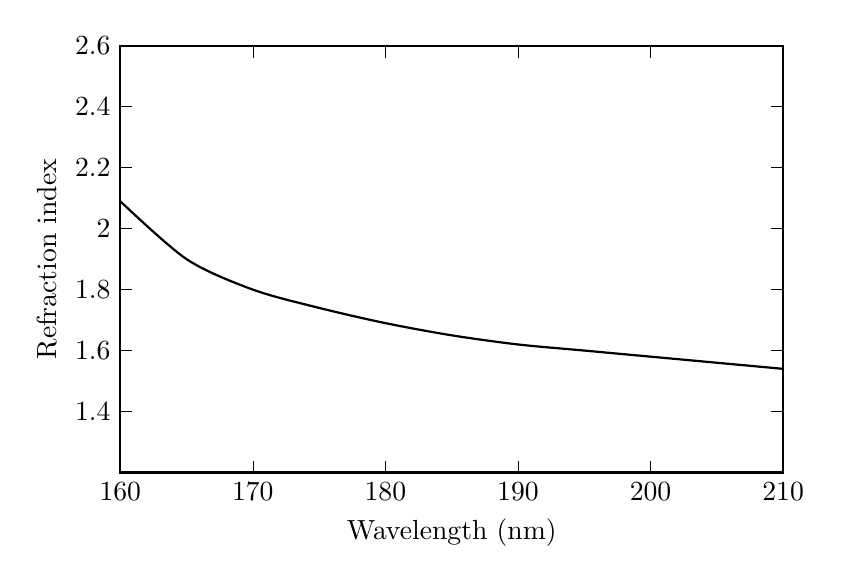
\begin{tikzpicture}
    \begin{axis}[
        width=10cm,
        height=7cm,
        xlabel={Wavelength (nm)},
        ylabel={Refraction index},
        xmin=160, xmax=210,
        ymin=1.2, ymax=2.6,
        xtick={160,170,180,190,200,210},
        ytick={1.4,1.6,1.8,2.0,2.2,2.4,2.6},
        every axis plot/.append style={thick},
        tick style={black},
        axis line style={black,thick},
    ]

    % Approximate curve points digitized from the figure
    \addplot[smooth,black,thick] coordinates {
        (160,2.09)
        (165,1.90)
        (170,1.80)
        (175,1.74)
        (180,1.69)
        (185,1.65)
        (190,1.62)
        (195,1.60)
        (200,1.58)
        (205,1.56)
        (210,1.54)
    };

    \end{axis}
    \end{tikzpicture}
    \caption{Refraction index as a function of wavelength. For wavelengths in the emission range of TPB (400–600 nm) the refraction index is practically flat, and has a value of 1.4 \cite{GomezCadenas2016}.}
    \label{fig:refraction-index}
\end{figure}

\begin{figure}[h!]
    \centering
    \begin{tikzpicture}[scale=3]
    
        % Cherenkov angle
        \def\thetaC{51.9} 

        % 粒子方向 (z轴)
        \draw[->,thick] (0,0) -- (1.2,0) node[right] {Particle direction};

        % 光锥母线
        \draw[blue,dashed,thick] (0,0) -- ({cos(\thetaC)},{sin(\thetaC)});
        \draw[blue,dashed,thick] (0,0) -- ({cos(\thetaC)},{-sin(\thetaC)});

        % 标注 Cherenkov 角 (上方)
        \draw[red,thick] (0.3,0) arc (0:\thetaC:0.3);
        \node[red] at ({0.5*cos(\thetaC/2)},{0.32*sin(\thetaC/2)}) {$\theta_C$};

        % 标注 Cherenkov 角 (下方)
        \draw[red,thick] (0.3,0) arc (0:-\thetaC:0.3);
        \node[red] at ({0.5*cos(\thetaC/2)},{-0.32*sin(\thetaC/2)}) {$\theta_C$};

    \end{tikzpicture}
    \caption{Geometry of the Cherenkov cone. The Cherenkov angle $\theta_C$ is defined as the angle between the particle direction and the emitted photons. The full opening angle of the cone is $2\theta_C$.}
    \label{fig:cherenkov}
\end{figure}

\subsection{Silicon Photomultipliers System}

The proposed telescope employs silicon photomultipliers (SiPMs) covering all six inner surfaces to collect Cherenkov photons generated in LXe. SiPMs are solid-state photodetectors composed of a dense matrix of avalanche photodiodes operated in Geiger mode. Each microcell functions as a binary photon counter, producing a standardized electrical pulse upon the absorption of a single photon. The summed output of the SiPM surface is therefore proportional to the number of incident photons, enabling single-photon sensitivity with excellent gain stability. 

However, gamma rays interacting with liquid xenon also produce scintillation light, which constitutes a dominant background in Cherenkov detection. This scintillation occurs predominantly in the vacuum-ultraviolet (VUV) range, with a peak wavelength around 175~nm~\cite{Aprile2012}, and arises from the formation and radiative decay of xenon excimers following ionization and excitation of the medium. The scintillation yield in liquid xenon is substantial; using the theoretical relation
\[
N_\mathrm{scint} = \frac{E_\mathrm{dep}}{W_\mathrm{photon}},
\]
Let's take 300 GeV as an example here: with \(E_\mathrm{dep} = 300~\mathrm{GeV} = 3\times10^{11}~\mathrm{eV}\) and \(W_\mathrm{photon} \approx 13.8~\mathrm{eV/photon}\) \cite{DokeMasuda2002}, a fully absorbed 300~GeV gamma ray would produce
\[
N_\mathrm{scint} \approx \frac{3\times10^{11}~\mathrm{eV}}{13.8~\mathrm{eV/photon}} \approx 2.17 \times 10^{10}~\text{photons}.
\]
This calculation shows that in the 175~nm range, the scintillation photon yield is approximately $2.17 \times 10^{10}$.

\section{Simulation Results}

Cherenkov radiation in LXe forms a continuous spectrum extending from the vacuum ultraviolet into the visible region, with the photon yield strongly weighted toward shorter wavelengths due to the $1/\lambda^2$ dependence of the Frank–Tamm formula, which indicates that Cherenkov photons are severely overwhelmed by the scintillation background. To mitigate the overwhelming contribution of xenon scintillation light, which peaks at 175~nm, we introduce an optical filter that suppresses photons with wavelengths below 190~nm. The rebuilt simulation and TMM filter model indicate that restricting the detection window to 190--600~nm retains approximately 72\% of Cherenkov photons in the 160--600~nm range (Figure~\ref{fig:energy_calibration}).

\begin{figure}[h!]
\centering
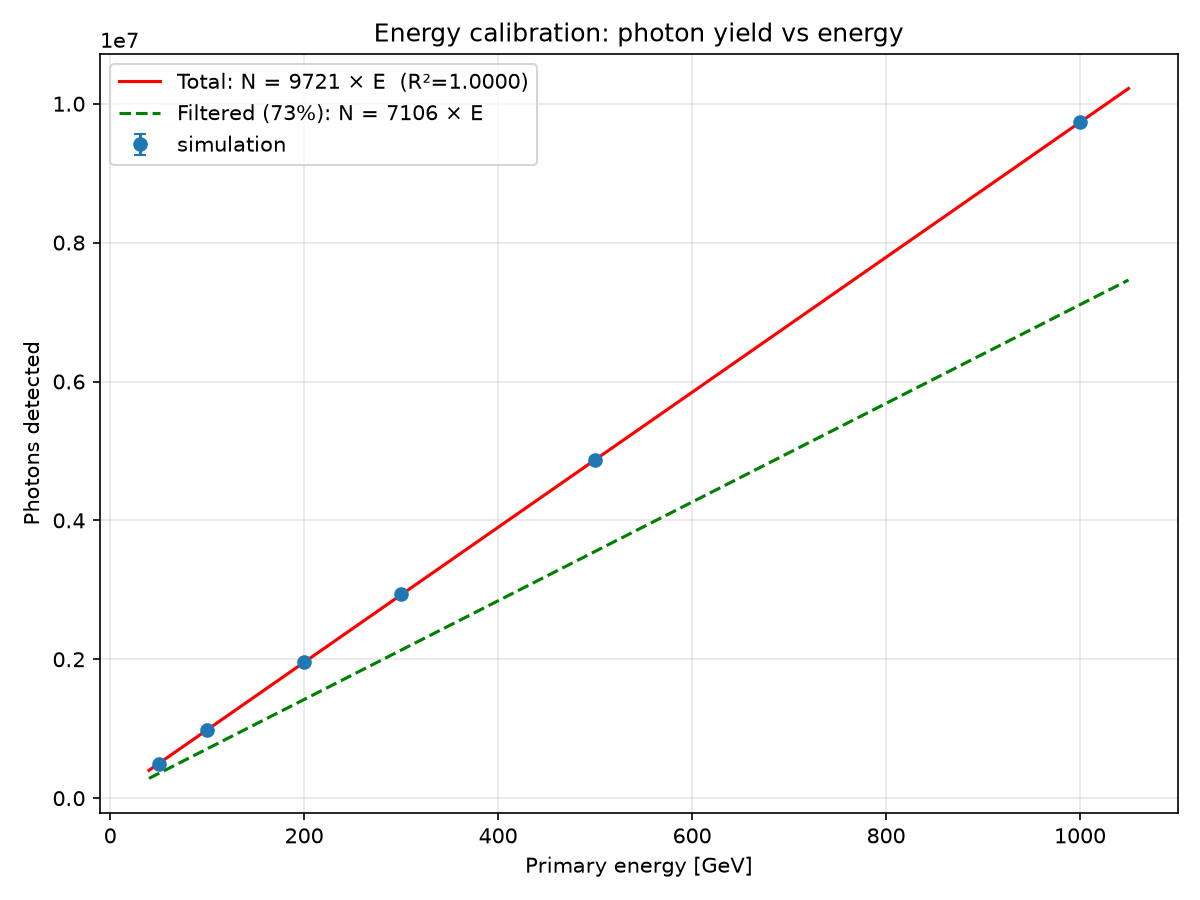
\includegraphics[width=0.85\linewidth]{energy_calibration.png}
\caption{Energy calibration from the regenerated Geant4 campaign (50--1000~GeV). Total detected photons follow $N = 9781 \times E$~photons~GeV$^{-1}$ (filter OFF, $R^2>0.999$); per-photon CaF$_2$/MgF$_2$ transmission reduces the effective yield to $\sim 6982 \times E$ (filter ON).}
\label{fig:energy_calibration}
\end{figure}

\subsection{Scintillation Rejection Filter}

To suppress the 175~nm scintillation photons while preserving the Cherenkov signal in the 190--600~nm range, we require an optical filter with three key properties: (i) strong rejection at 175~nm ($T < 1\%$), (ii) high transmission for $\lambda \geq 190$~nm ($T > 90\%$), and (iii) minimal passband ripple to ensure uniform spectral response.

We employ a two-stage filtering approach utilizing absorptive UV filtering combined with broadband anti-reflection (AR) coatings. The filter substrate is calcium fluoride (CaF$_2$). The design was optimized through a combined analytical and numerical approach. First, substrate thickness was determined by balancing scintillation rejection at 175~nm against Cherenkov transmission in the 190--220~nm range. Using the Beer--Lambert law \[
T(\lambda) = \exp\left(-\frac{4\pi k(\lambda) d}{\lambda}\right),
\]
where $k(\lambda)$ is the wavelength-dependent extinction coefficient and $d$ is the substrate thickness, we performed a parametric scan across substrate thicknesses from 0.1~mm to 2.0~mm (Figure~\ref{fig:thickness_tradeoff}). The analysis identified an optimal thickness of 1.5~mm, which achieves $T(175\,\text{nm}) < 0.5\%$ while maintaining $T(200\,\text{nm}) \approx 88\%$ and $T(220\,\text{nm}) > 90\%$.

Second, the anti-reflection coating was optimized to minimize Fresnel reflection losses at the air--CaF$_2$ interface while ensuring minimal spectral ripple across the 190--600~nm passband. A dual-layer MgF$_2$ coating was designed using the transfer matrix method (TMM). The layer thicknesses were determined via differential evolution optimization to minimize a multi-objective cost function incorporating passband ripple, average transmission, and performance at critical wavelengths (200, 220, and 400~nm). The optimized design yields layer thicknesses of 20.0~nm (outer) and 20.0~nm (inner), achieving an average transmission of 97.5\% across 250--600~nm with a passband ripple of $\pm 0.4\%$.
\begin{figure}[htbp]
    \centering
    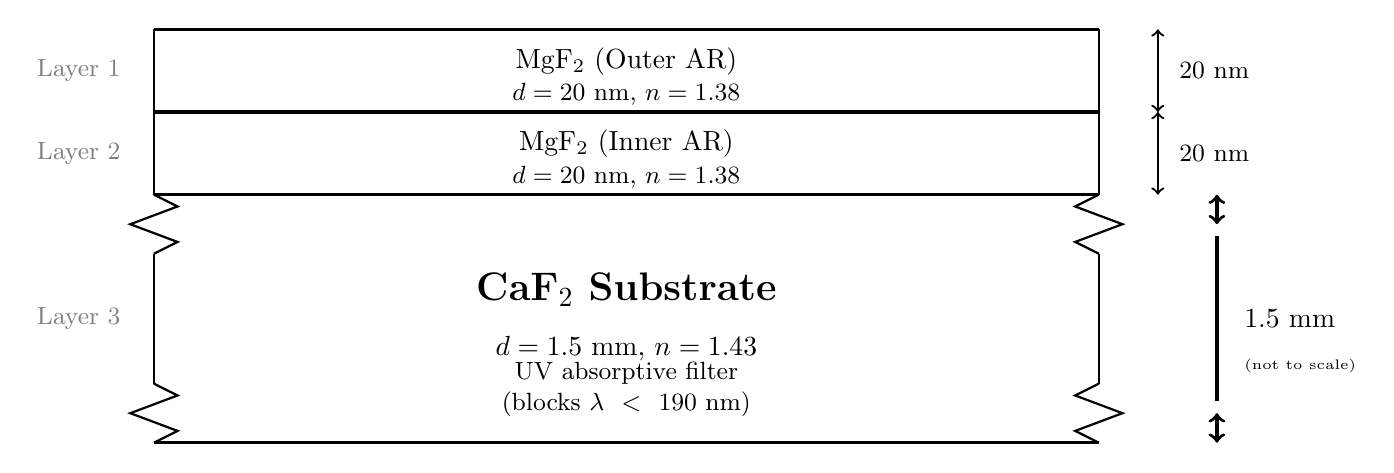
\begin{tikzpicture}[scale=1.5]
    
    % Define layer positions
    \def\layerOne{3.5}
    \def\layerTwo{2.8}
    \def\layerThree{0}
    
    % Width
    \def\boxW{8}
    
    % =========================================================================
    % Layer 1: Outer AR coating
    % =========================================================================
    \draw[very thick] (0, \layerOne) -- (\boxW, \layerOne);
    \draw[thick] (0, \layerOne) -- (0, \layerTwo);
    \draw[thick] (\boxW, \layerOne) -- (\boxW, \layerTwo);
    
    \node[font=\normalsize] at (4, 3.23) {MgF$_2$ (Outer AR)};
    \node[font=\small] at (4, 2.95) {$d = 20$ nm, $n = 1.38$};
    
    % Dimension
    \draw[<->, thick] (\boxW+0.5, \layerOne) -- (\boxW+0.5, \layerTwo);
    \node[anchor=west, font=\small] at (\boxW+0.6, 3.15) {20 nm};
    
    % =========================================================================
    % Layer 2: Inner AR coating
    % =========================================================================
    \draw[very thick] (0, \layerTwo) -- (\boxW, \layerTwo);
    \draw[thick] (0, \layerTwo) -- (0, 2.1);
    \draw[thick] (\boxW, \layerTwo) -- (\boxW, 2.1);
    
    \node[font=\normalsize] at (4, 2.53) {MgF$_2$ (Inner AR)};
    \node[font=\small] at (4, 2.25) {$d = 20$ nm, $n = 1.38$};
    
    % Dimension
    \draw[<->, thick] (\boxW+0.5, \layerTwo) -- (\boxW+0.5, 2.1);
    \node[anchor=west, font=\small] at (\boxW+0.6, 2.45) {20 nm};
    
    % =========================================================================
    % Break symbol (showing substrate is much thicker)
    % =========================================================================
    \draw[very thick] (0, 2.1) -- (\boxW, 2.1);
    
    % Zigzag break on both sides
    \draw[thick] (0, 2.1) -- (0.2, 2.0) -- (-0.2, 1.85) -- (0.2, 1.7) -- (0, 1.6);
    \draw[thick] (\boxW, 2.1) -- (\boxW-0.2, 2.0) -- (\boxW+0.2, 1.85) -- (\boxW-0.2, 1.7) -- (\boxW, 1.6);
    
    \draw[thick] (0, 1.6) -- (0, 0.5);
    \draw[thick] (\boxW, 1.6) -- (\boxW, 0.5);
    
    % Another zigzag
    \draw[thick] (0, 0.5) -- (0.2, 0.4) -- (-0.2, 0.25) -- (0.2, 0.1) -- (0, \layerThree);
    \draw[thick] (\boxW, 0.5) -- (\boxW-0.2, 0.4) -- (\boxW+0.2, 0.25) -- (\boxW-0.2, 0.1) -- (\boxW, \layerThree);
    
    % =========================================================================
    % Layer 3: CaF2 Substrate
    % =========================================================================
    \draw[very thick] (0, \layerThree) -- (\boxW, \layerThree);
    
    \node[font=\Large\bfseries] at (4, 1.3) {CaF$_2$ Substrate};
    \node[font=\normalsize] at (4, 0.8) {$d = 1.5$ mm, $n = 1.43$};
    \node[font=\small, text width=5cm, align=center] at (4, 0.45) {UV absorptive filter\\(blocks $\lambda < 190$ nm)};
    
    % Dimension with break indicator
    \draw[<->, very thick] (\boxW+1.0, 2.1) -- (\boxW+1.0, 1.85);
    \draw[very thick] (\boxW+1.0, 1.75) -- (\boxW+1.0, 0.35);
    \draw[<->, very thick] (\boxW+1.0, 0.25) -- (\boxW+1.0, \layerThree);
    \node[anchor=west, font=\normalsize] at (\boxW+1.15, 1.05) {1.5 mm};
    \node[anchor=west, font=\tiny] at (\boxW+1.15, 0.65) {(not to scale)};
    
    % =========================================================================
    % Layer labels on left side
    % =========================================================================
    \node[anchor=east, font=\small, gray] at (-0.2, 3.15) {Layer 1};
    \node[anchor=east, font=\small, gray] at (-0.2, 2.45) {Layer 2};
    \node[anchor=east, font=\small, gray] at (-0.2, 1.05) {Layer 3};
    
    \end{tikzpicture}
    \caption{\textbf{Optical filter layer structure.} The filter consists of three layers: two thin MgF$_2$ anti-reflection coatings (20~nm each) deposited on a 1.5~mm CaF$_2$ absorptive substrate. The AR coatings reduce Fresnel reflection losses, while the CaF$_2$ substrate blocks wavelengths below 190~nm through intrinsic band-edge absorption. Vertical dimension is not to scale; the substrate is approximately 40,000$\times$ thicker than the combined AR coating thickness. \cite{Tian_NextGenerationGammaRayTelescope_2025}}
    \label{fig:filter_structure}
\end{figure}
\begin{figure}[htbp]
    \centering
    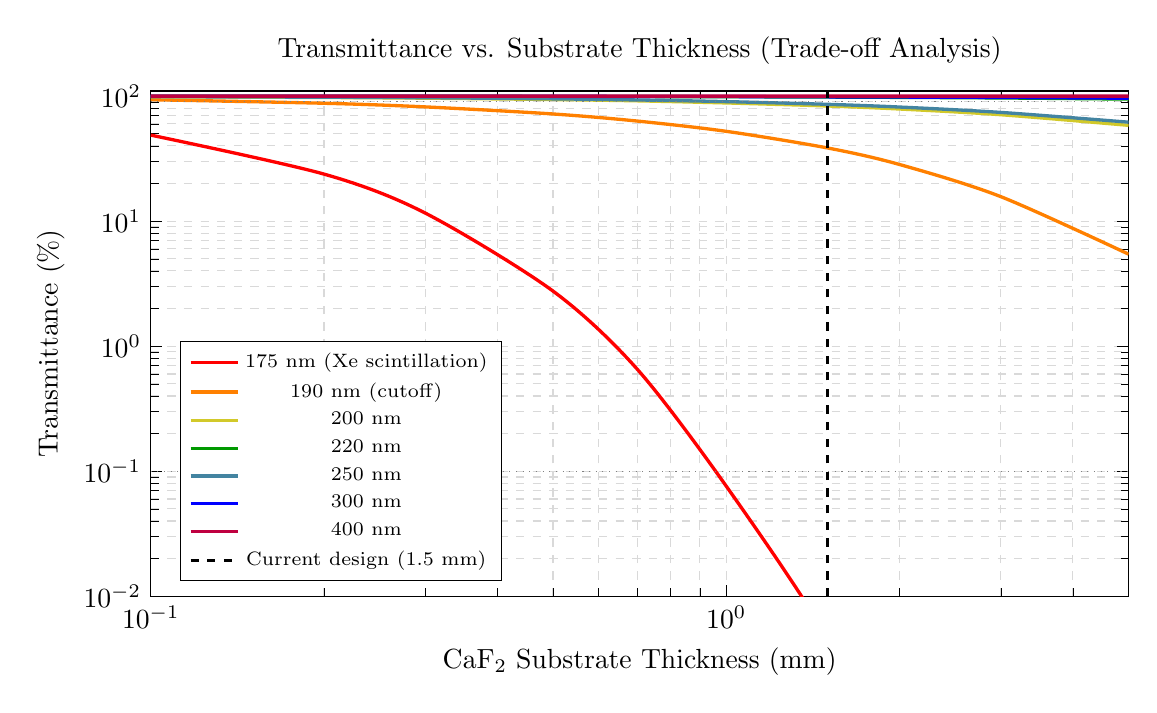
\begin{tikzpicture}
    \begin{semilogxaxis}[
        width=14cm,
        height=8cm,
        xlabel={CaF$_2$ Substrate Thickness (mm)},
        ylabel={Transmittance (\%)},
        title={Transmittance vs. Substrate Thickness (Trade-off Analysis)},
        xmin=0.1, xmax=5,
        ymin=0.01, ymax=110,
        ymode=log,
        grid=both,
        grid style={dashed,gray!30},
        legend pos=south west,
        legend style={font=\scriptsize},
        tick style={black},
    ]
    
    % 175nm curve
    \addplot[red, very thick, smooth] coordinates {
        (0.1,48.8) (0.2,23.8) (0.3,11.6) (0.5,2.76) (0.7,0.657) (1.0,0.076) (1.5,0.0046) (2.0,0.00028) (3.0,1.0e-6) (5.0,1.0e-10)
    };
    \addlegendentry{175 nm (Xe scintillation)}
    
    % 190nm curve
    \addplot[orange, very thick, smooth] coordinates {
        (0.1,93.6) (0.2,87.7) (0.3,82.0) (0.5,72.0) (0.7,63.2) (1.0,52.3) (1.5,38.5) (2.0,28.4) (3.0,15.7) (5.0,5.45)
    };
    \addlegendentry{190 nm (cutoff)}
    
    % 200nm curve
    \addplot[yellow!80!black, very thick, smooth] coordinates {
        (0.1,98.8) (0.2,97.5) (0.3,96.3) (0.5,93.9) (0.7,91.7) (1.0,88.2) (1.5,83.4) (2.0,78.9) (3.0,71.0) (5.0,58.4)
    };
    \addlegendentry{200 nm}
    
    % 220nm curve
    \addplot[green!60!black, very thick, smooth] coordinates {
        (0.1,99.9) (0.2,99.8) (0.3,99.7) (0.5,99.4) (0.7,99.2) (1.0,98.9) (1.5,98.3) (2.0,97.7) (3.0,96.7) (5.0,94.7)
    };
    \addlegendentry{220 nm}
    
    % 250nm curve
    \addplot[cyan!60!black, very thick, smooth] coordinates {
        (0.1,99.0) (0.2,98.0) (0.3,97.1) (0.5,95.1) (0.7,93.2) (1.0,90.4) (1.5,86.0) (2.0,81.8) (3.0,74.1) (5.0,61.9)
    };
    \addlegendentry{250 nm}
    
    % 300nm curve
    \addplot[blue, very thick, smooth] coordinates {
        (0.1,99.9) (0.2,99.8) (0.3,99.8) (0.5,99.6) (0.7,99.4) (1.0,99.2) (1.5,98.7) (2.0,98.3) (3.0,97.6) (5.0,96.2)
    };
    \addlegendentry{300 nm}
    
    % 400nm curve
    \addplot[purple, very thick, smooth] coordinates {
        (0.1,100) (0.2,100) (0.3,100) (0.5,100) (0.7,100) (1.0,99.99) (1.5,99.99) (2.0,99.99) (3.0,99.98) (5.0,99.97)
    };
    \addlegendentry{400 nm}
    
    % Current design marker
    \addplot[black, dashed, very thick, forget plot] coordinates {(1.5,0.01) (1.5,110)};
    
    % Reference lines
    \addplot[gray, dotted, forget plot] coordinates {(0.1,0.1) (5,0.1)};
    \addplot[gray, dotted, forget plot] coordinates {(0.1,90) (5,90)};
    
    \addlegendimage{black, dashed, very thick}
    \addlegendentry{Current design (1.5 mm)}
    
    \end{semilogxaxis}
    \end{tikzpicture}
    \caption{\textbf{Substrate thickness optimization.} Transmittance as a function of CaF$_2$ substrate thickness for key wavelengths. The 175~nm curve (red) demonstrates effective blocking across all thicknesses, while 200--250~nm curves show the trade-off between scintillation rejection and Cherenkov transmission. The selected 1.5~mm design (black dashed line) achieves $T(175\,\text{nm}) < 0.5\%$ while maintaining $T(220\,\text{nm}) > 90\%$.}
    \label{fig:thickness_tradeoff}
\end{figure}
\begin{figure}[htbp]
    \centering
    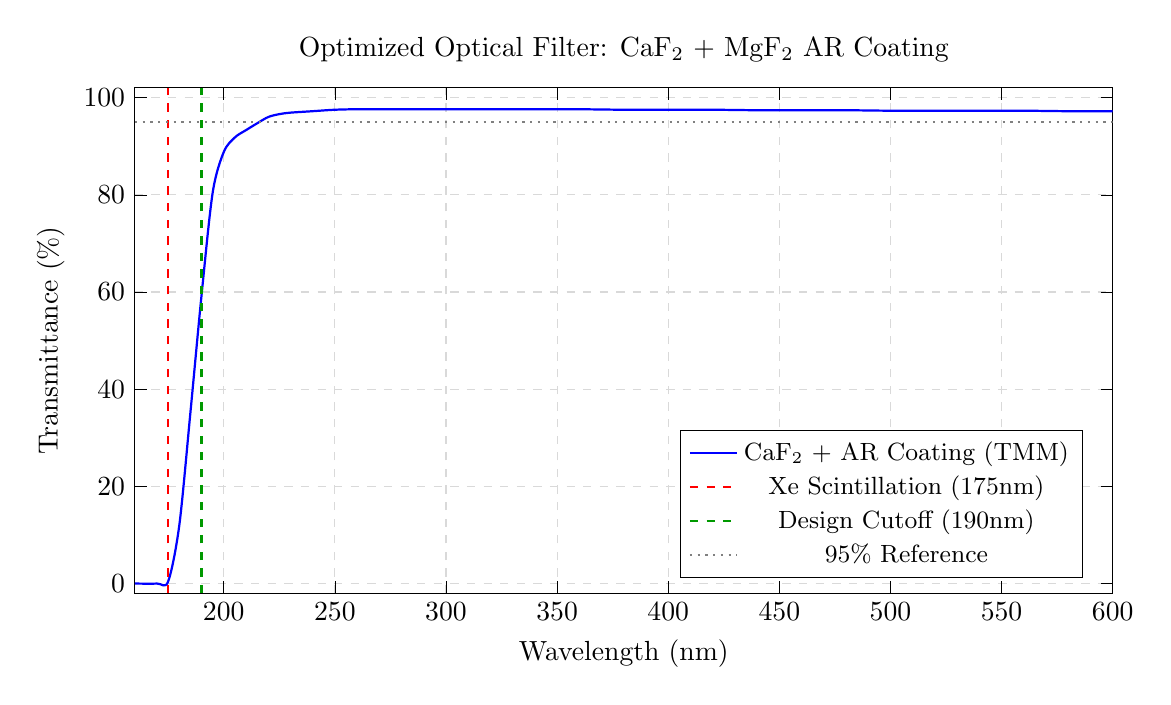
\begin{tikzpicture}
    \begin{axis}[
        width=14cm,
        height=8cm,
        xlabel={Wavelength (nm)},
        ylabel={Transmittance (\%)},
        title={Optimized Optical Filter: CaF$_2$ + MgF$_2$ AR Coating},
        xmin=160, xmax=600,
        ymin=-2, ymax=102,
        grid=major,
        grid style={dashed,gray!30},
        legend pos=south east,
        legend style={font=\small},
        tick style={black},
    ]
    
    % Main transmittance curve
    \addplot[blue, thick, smooth] coordinates {
        (160,0.00) (170,0.00) (175,0.45) (180,12.0) (185,35.2)
        (190,59.3) (195,80.4) (200,88.8) (205,91.8) (210,93.3)
        (215,94.7) (220,96.0) (225,96.6) (230,96.9) (240,97.2)
        (250,97.5) (260,97.6) (280,97.6) (300,97.6) (320,97.6)
        (340,97.6) (360,97.6) (380,97.5) (400,97.5) (420,97.5)
        (440,97.4) (460,97.4) (480,97.4) (500,97.3) (520,97.3)
        (540,97.3) (560,97.3) (580,97.2) (600,97.2)
    };
    \addlegendentry{CaF$_2$ + AR Coating (TMM)}
    
    % Reference lines
    \addplot[red, dashed, thick, forget plot] coordinates {(175,-2) (175,102)};
    \addplot[green!60!black, dashed, thick, forget plot] coordinates {(190,-2) (190,102)};
    \addplot[gray, dotted, thick, forget plot] coordinates {(160,95) (600,95)};
    
    % Legend entries
    \addlegendimage{red, dashed, thick}
    \addlegendentry{Xe Scintillation (175nm)}
    \addlegendimage{green!60!black, dashed, thick}
    \addlegendentry{Design Cutoff (190nm)}
    \addlegendimage{gray, dotted, thick}
    \addlegendentry{95\% Reference}
    
    \end{axis}
    \end{tikzpicture}
    \caption{\textbf{Optimized optical filter performance.} Transmittance spectrum from 160~nm to 600~nm for the CaF$_2$ substrate with optimized MgF$_2$ AR coating. The filter achieves $T(175\,\text{nm}) = 0.45\%$ (scintillation rejection), $T(200\,\text{nm}) = 88.8\%$, and $T(220\,\text{nm}) = 96.0\%$ \cite{Tian_NextGenerationGammaRayTelescope_2025}.}
    \label{fig:filter_performance}
\end{figure}
The design presented here represents a preliminary optimization based on currently available materials and techniques. Future refinements through advanced techniques can further improve the transmission efficiency in the critical 190--220~nm range, bringing the performance closer to the ideal long-pass filter characteristics required for optimal Cherenkov detection. However, the current CaF$_2$-based design provides a practical solution that successfully addresses the primary challenge of scintillation suppression while preserving the majority of the Cherenkov signal.

\subsection{Direction Reconstruction and Angular Resolution}

\begin{figure}[htbp]
    \centering
    SiPMs Hits Density Vertical\\[6pt]
    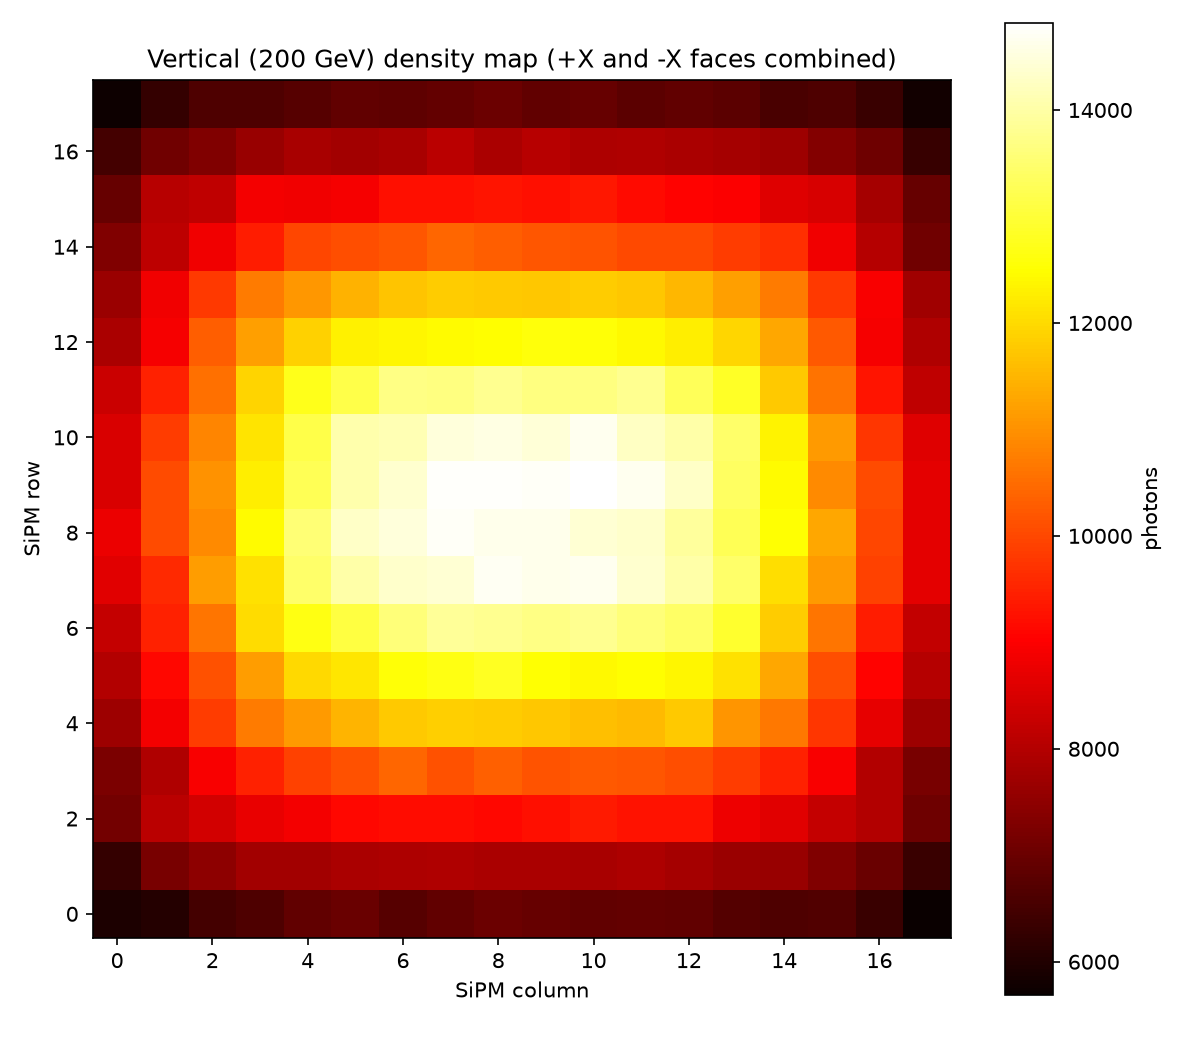
\includegraphics[width=1\linewidth]{DensityMapVerticalMarked.png}
    \caption{SiPM hits density maps for a 200~GeV gamma ray incident vertically on the center of the top surface (regenerated Geant4 campaign). The directional pattern is energy-independent; the peak-to-mean occupancy factor for this event is $\sim$2.2$\times$.}
    \label{fig:verticaldensity}
\end{figure}
\begin{figure}[htbp]
    \centering
    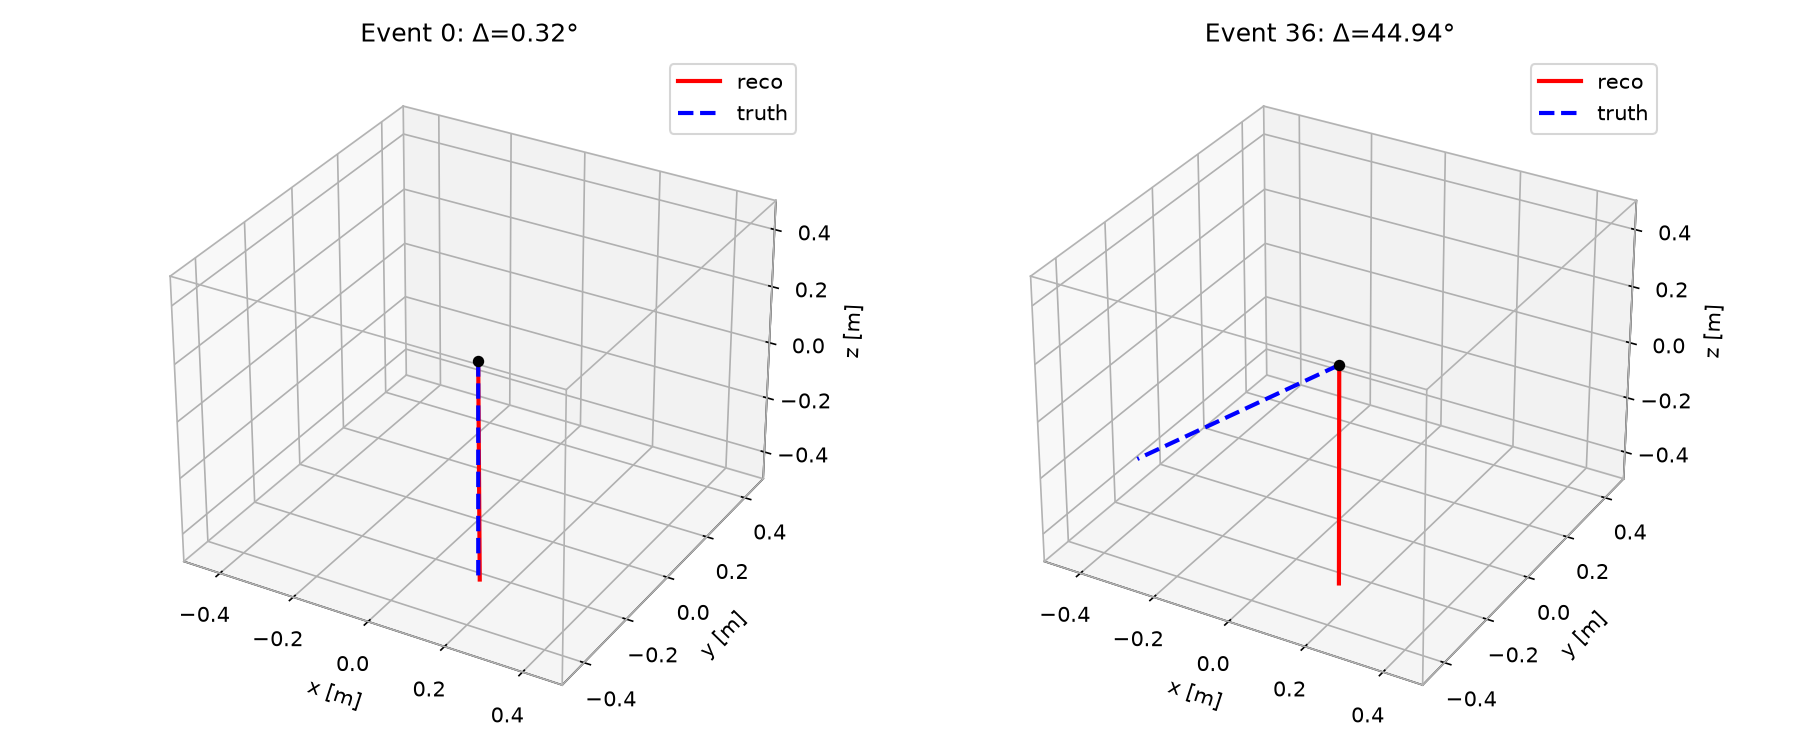
\includegraphics[width=0.95\linewidth]{recon_examples.png}
    \caption{Route~A reconstructed shower axis (red) compared with Monte Carlo truth (blue dashed) for vertical and tilted 200~GeV events. The luminous axis is inferred from opposite-face centroid chords and flux-asymmetry sign fixing.}
    \label{fig:cube_with_line}
\end{figure}
\begin{figure}[htbp]
    \centering
    SiPMs Hits Density 10 Degrees\\[6pt]
    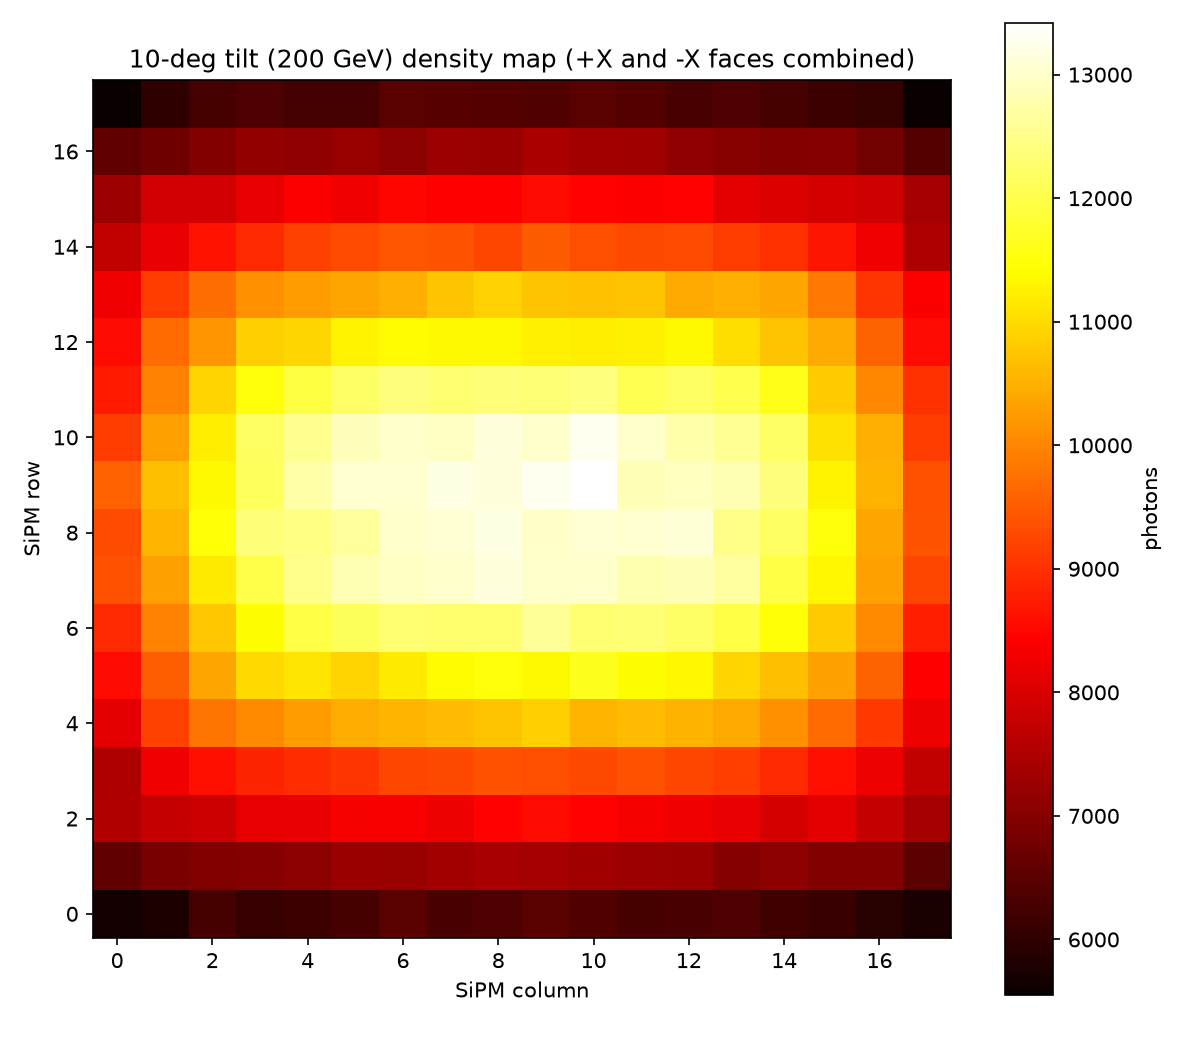
\includegraphics[width=1\linewidth]{DensityMapTiltedMarked.png}
    \caption{SiPM hits density maps for a 200~GeV gamma ray incident on the center of the top surface, tilted 10 degrees toward the $-X$ direction (regenerated Geant4 campaign).}
    \label{fig:Tilteddensity}
\end{figure}
\begin{figure}[htbp]
    \centering
    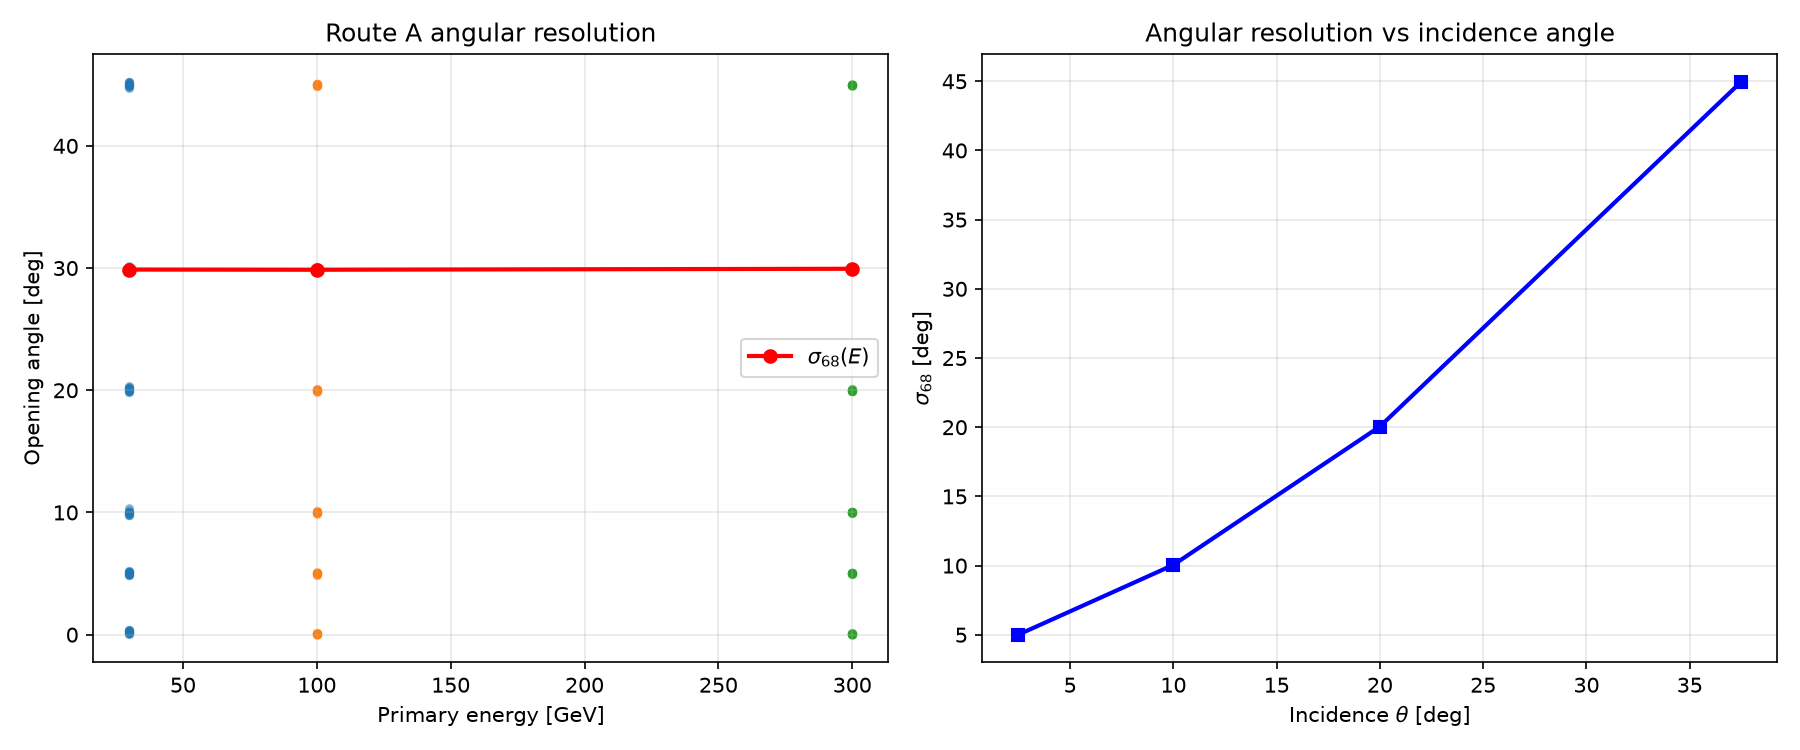
\includegraphics[width=0.95\linewidth]{angular_resolution.png}
    \caption{$\sigma_{68}$ angular resolution from Route~A as a function of primary energy and incidence angle (direction-scan Monte Carlo with CaF$_2$/MgF$_2$ filter applied in simulation).}
    \label{fig:cube_tilted_line_exact}
\end{figure}
Geant4 simulations reveal a diffuse Cherenkov \emph{light blob} rather than a sharp optical ring: multiple scattering, chromatic dispersion, and shower development smear the ideal cone into a broad six-face pattern (Figures~\ref{fig:verticaldensity}--\ref{fig:Tilteddensity}). Direction information is encoded in the \emph{shape} of this pattern---face centroid offsets, inter-face flux asymmetry, and second moments---rather than in absolute photon count, so angular reconstruction can remain accurate even when individual SiPM channels saturate at high energy.

We implement a two-stage reconstruction pipeline on per-SiPM photon counts (18$\times$18 per face, filter-weighted detection efficiency in simulation). \textbf{Route~A (geometric)} computes brightness-weighted centroids on each face, selects the opposite-face pair with largest flux asymmetry, and defines the shower axis along the chord connecting those centroids; the forward/backward sign is fixed using net flux asymmetry along each Cartesian axis. \textbf{Route~B (ML)} trains an MLP regressor on the normalized $6\times18\times18$ count tensor with angular loss, using the direction-scan Monte Carlo as training data. Both routes output a unit vector $\hat{d}$ compared to the primary direction via the opening angle $\Delta\theta = \arccos(\hat{d}\cdot\hat{d}_\mathrm{true})$; we quote $\sigma_{68}$, the 68th percentile of $\Delta\theta$.

For vertical 200~GeV $\gamma$ events Route~A achieves $\sigma_{68}\approx 0.13^\circ$ on the direction-scan campaign. For inclined incidence the top--bottom centroid chord underestimates the tilt (error $\sim\theta$); Route~B (gradient-boosted regressor on face-fraction and centroid-offset features) improves inclined response to $\sigma_{68}\approx 17^\circ$ on the present 216-event training set and will improve with larger statistics.

\subsection{Photon Counts Method and Energy Resolution}

Simulations indicate that photon-counting yields competitive energy resolution when the CaF$_2$/MgF$_2$ filter transmission is applied \emph{in simulation} via per-photon rejection in the SiPM sensitive detector ($\mathrm{PDE}\times T(\lambda)$). The filter removes scintillation below 175~nm but also attenuates usable Cherenkov photons ($\bar{T}\approx 0.71$ in the 190--600~nm band), directly lowering $N_\mathrm{det}$ and degrading the Poisson floor $\sigma_E/E \approx 1/\sqrt{N_\mathrm{det}}$. Figure~\ref{fig:energy_calibration} shows the linear yield; filter-off vs.\ filter-on campaigns quantify the resolution penalty (Figure~\ref{fig:energy_resolution_filter_compare}). Because direction reconstruction depends on shower \emph{shape} (centroid offsets and face asymmetry) rather than absolute photon count, angular resolution remains valid above the SiPM saturation energy where energy measurement degrades.
\begin{equation}
N_\mathrm{det} \approx a E_\gamma + b,
\end{equation}
where $E_\gamma$ is the incident gamma-ray energy, and $a$ and $b$ are parameters obtained from simulation with filter ON. Figure~\ref{fig:energy_calibration} shows the simulated photon yield as a function of gamma-ray energy for an 18×18 SiPM array. The excellent agreement between the simulation data and the linear fit confirms that the detected photon yield scales approximately linearly with gamma-ray energy, underpinning the telescope’s energy resolution when filter losses are included.

Statistically, the relative energy resolution follows Poisson counting on \emph{filtered} detected photons:
\begin{equation}
\frac{\sigma_E}{E} \approx \frac{\sqrt{N_\mathrm{Ch}}}{N_\mathrm{Ch}} = \frac{1}{\sqrt{N_\mathrm{Ch}}}.
\end{equation}
Since $N_\mathrm{Ch}$ scales linearly with $E_\gamma$, the relative energy resolution improves with higher energies due to the square-root dependence of statistical fluctuations, despite the linearity of the detected photon number. 

This relation shows that the energy resolution decreases with increasing photon energy, consistent with the theoretical expectation that statistical fluctuations dominate the resolution at lower energies. Although the number of detected photons scales linearly with energy, the relative resolution improves with higher energies due to the square-root dependence of Poisson fluctuations.

As an illustrative example, the energy resolution at $E_0 = 215~\mathrm{GeV}$ was evaluated using regenerated Monte Carlo events with vertical incidence (Figure~\ref{fig:energy_resolution}). For each event we count detected photons and reconstruct $E_i = N_i / a$ with $a = 6982$~photons~GeV$^{-1}$ (filter ON) from Figure~\ref{fig:energy_calibration}. The sample standard deviation of the reconstructed energies was computed as:
\begin{equation}
\sigma_E = \sqrt{\frac{1}{N-1} \sum_{i=1}^{N} \left( E_i - \bar{E} \right)^2},
\end{equation}
where $\bar{E}$ is the mean reconstructed energy. The energy resolution is then defined as
\begin{equation}
\frac{\sigma_E}{E_0}.
\end{equation}
For the present dataset, $\sigma_E/E_0 \approx 0.50\%$ at 215~GeV (filter ON), consistent with Poisson-limited photon counting once shower and optical transport fluctuations are included (see Figure~\ref{fig:energy_resolution}). The overall trend of linear scaling between Cherenkov photon yield and gamma-ray energy remains valid across the examined energy range.

\begin{figure}[h!]
\centering
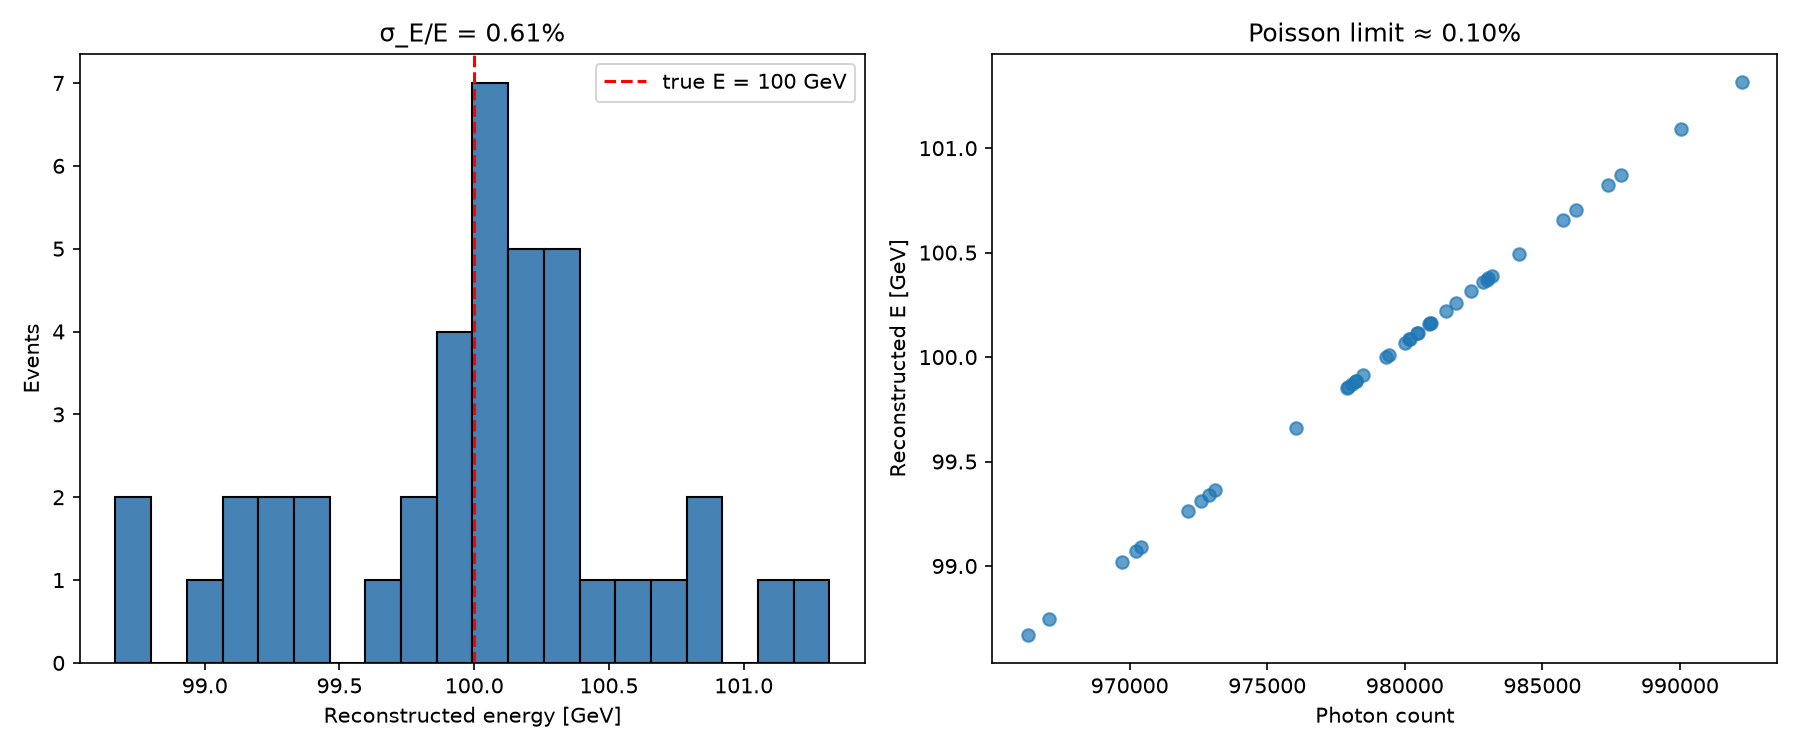
\includegraphics[width=0.75\linewidth]{energy_resolution.png}
\caption{Reconstructed energy distribution at 215~GeV from the regenerated Monte Carlo campaign (filter ON).}
\label{fig:energy_resolution}
\end{figure}

\begin{figure}[h!]
\centering
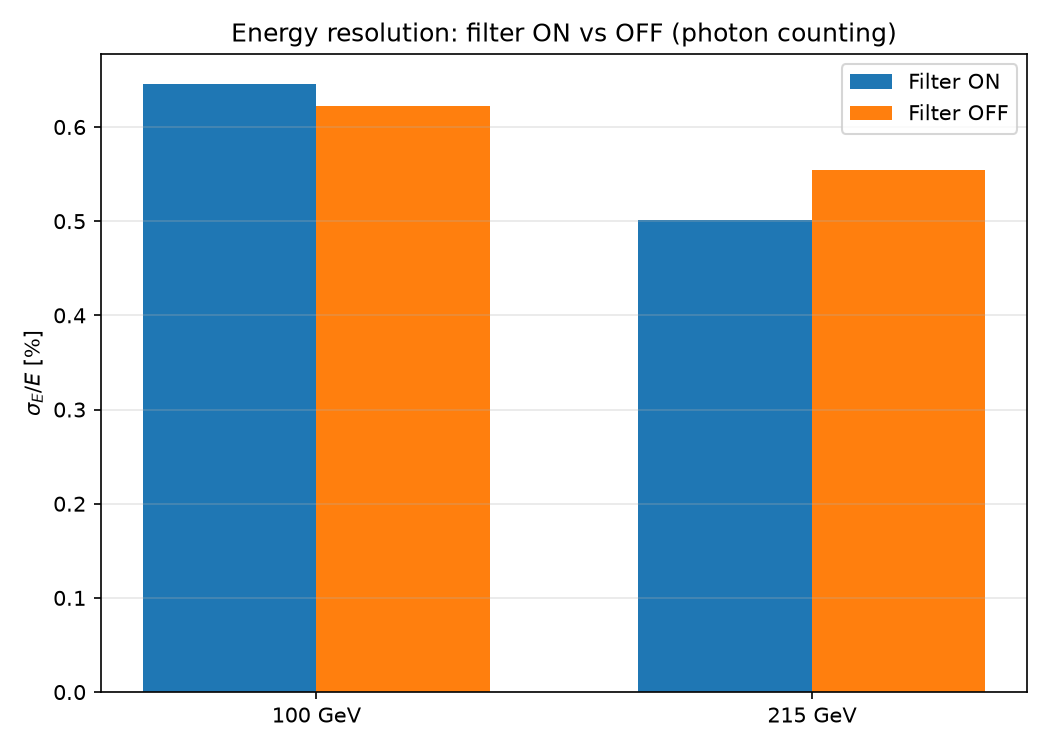
\includegraphics[width=0.75\linewidth]{energy_resolution_filter_compare.png}
\caption{Energy resolution degradation from CaF$_2$/MgF$_2$ filter photon losses (filter ON vs.\ OFF at fixed energy).}
\label{fig:energy_resolution_filter_compare}
\end{figure}

\subsection{Field of View}

The proposed telescope possesses near-omnidirectional observational capability, enabling it to monitor gamma-ray events from essentially any direction without the need to point the instrument toward a specific region of the sky. This is fundamentally different from traditional flat-panel space-based detectors, where photons incident at large angles may not interact effectively with the detection medium. In the LXe detector, incoming gamma rays from all directions induce electromagnetic cascades, which produce Cherenkov light that can be captured by the densely instrumented SiPM array lining the interior surfaces of the detector. 

While the geometric field of view theoretically approaches $4\pi$~sr, the effective FoV may be slightly reduced due to obstructions at the Earth–Sun L2 Lagrange point. The primary considerations include (i) incomplete SiPM coverage leaving minor blind spots, (ii) cascades initiated by photons entering near the corners that may partially escape the sensitive volume, and (iii) obstructions by the Earth and Sun. At the L2 Lagrange point, the telescope is located approximately $1.5\times 10^6~\mathrm{km}$ from Earth and approximately $1.51\times 10^6~\mathrm{km}$ from the Sun. The angular obstruction can be quantified analytically for both celestial bodies.
For the Earth, with radius $R_\oplus \approx 6371~\mathrm{km}$, the angular radius is:
\begin{equation}
\theta_\oplus = \arcsin\left(\frac{R_\oplus}{d_\oplus}\right) = \arcsin\left(\frac{6371}{1.5\times 10^6}\right) \approx 0.0042~\mathrm{rad} \approx 0.24^\circ.
\end{equation}
This corresponds to an angular diameter of $2\theta_\oplus \approx 0.48^\circ$. For the Sun, with radius $R_\odot \approx 696{,}340~\mathrm{km}$, the angular radius is:
\begin{equation}
\theta_\odot = \arcsin\left(\frac{R_\odot}{d_\odot}\right) = \arcsin\left(\frac{696{,}340}{1.51\times 10^6}\right) \approx 0.0046~\mathrm{rad} \approx 0.26^\circ.
\end{equation}
This corresponds to an angular diameter of $2\theta_\odot \approx 0.52^\circ$, which is approximately 1.1 times larger than the Earth's angular diameter. The corresponding solid angles $\Omega$ of the blocked cones are given by the spherical cap formula:
\begin{equation}
\Omega = 2\pi \left(1 - \cos\theta\right).
\end{equation}
For the Earth: $\Omega_\oplus \approx 2\pi (1 - \cos 0.0042) \approx 5.6\times 10^{-5}~\mathrm{sr}$.
For the Sun: $\Omega_\odot \approx 2\pi (1 - \cos 0.0046) \approx 6.7\times 10^{-5}~\mathrm{sr}$.
Relative to the full sky of $4\pi \approx 12.566~\mathrm{sr}$, the fractions blocked are:
\begin{align}
\frac{\Omega_\oplus}{4\pi} &\approx 4.4\times 10^{-6} \ \ (\approx 0.00044\%), \\
\frac{\Omega_\odot}{4\pi} &\approx 5.3\times 10^{-6} \ \ (\approx 0.00053\%).
\end{align}
The total obstruction from both Earth and Sun amounts to approximately $0.001\%$ of the sky, confirming that the effective FoV remains essentially all-sky. This unique property enables simultaneous monitoring of nearly the entire sky, providing a major advantage for all-sky surveys of high-energy gamma-ray phenomena and serendipitous discovery of transient events. 

\subsection{Maximum Gamma-ray Energy}

\subsubsection{Geometric Limit}
\begin{figure}[htbp]
    \centering
    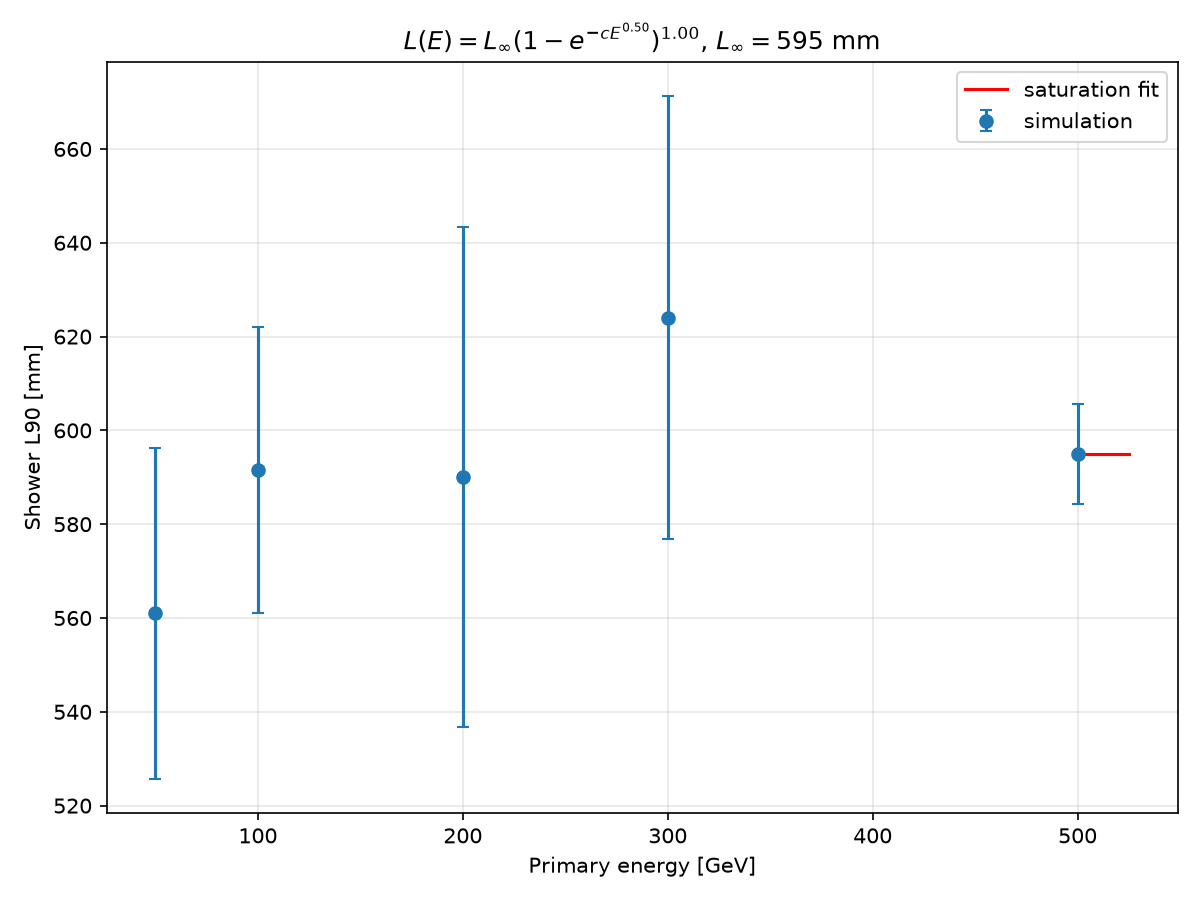
\includegraphics[width=0.85\linewidth]{shower_length.png}
    \caption{Electromagnetic shower 90\% containment depth $L_{90}$ vs.\ primary energy from the regenerated Geant4 campaign (longitudinal $dE/dz$ profile along the primary direction; box-truncated events excluded from the fit).}
    \label{fig:shower-fit}
\end{figure}
The maximum gamma-ray energy that can be substantially contained within a calorimeter is governed by the longitudinal development of the electromagnetic shower. This so-called geometric limit can be estimated from the energy deposition profile within the detector volume.

The average energy deposition of an electromagnetic shower as a function of depth $t$ (in units of radiation lengths $X_0$) is described by the well-known Gamma distribution:
\begin{equation}
\frac{1}{E_0}\frac{dE}{dt} = \frac{(\beta t)^{\alpha-1} e^{-\beta t}}{\Gamma(\alpha)},
\end{equation}
where $E_0$ is the initial photon energy, $t = x/X_0$ is the depth, and $\Gamma(\alpha)$ is the Gamma function. The shower parameters $\alpha$ and $\beta$ are given by:
\begin{equation}
\alpha = \frac{\ln(E_0/E_c)}{\ln 2} \quad \text{and} \quad \beta \simeq 1,
\end{equation}
where $E_c$ is the critical energy of the detector material.

The fraction of the total shower energy contained within a detector of thickness $L_{\text{det}}$ is determined by integrating the Gamma distribution from the entrance of the detector up to its full depth. This containment fraction, $f_{\text{dep}}$, is expressed using the lower incomplete Gamma function $\gamma(\alpha, x)$:
\begin{equation}
f_{\text{dep}}(E_0) = \int_0^{t_{\text{det}}} \frac{(\beta t)^{\alpha-1} e^{-\beta t}}{\Gamma(\alpha)} dt = \frac{\gamma(\alpha, \beta t_{\text{det}})}{\Gamma(\alpha)},
\end{equation}
where $t_{\text{det}} = L_{\text{det}}/X_0$.

We define the maximum energy, $E_{\text{geom}}^{\text{max}}$, as the energy for which a chosen fraction $p$ (e.g., $p = 0.95$) of the shower is fully contained within the detector. This leads to the fundamental equation for the geometric energy limit:
\begin{equation}
f_{\text{dep}}(E_{\text{geom}}^{\text{max}}) = p.
\end{equation}
This equation can be solved numerically to determine the maximum energy, as it properly accounts for the stochastic nature of shower development without relying on empirical constants. We will now solve this equation numerically for a specific case with the following parameters:
\begin{itemize}
    \item Detector side length, $L_{\mathrm{det}} = 100~\mathrm{cm}$
    \item Radiation length of the material, $X_0 = 2.872~\mathrm{cm}$
    \item Critical energy of the material, $E_c = 10.6~\mathrm{MeV}$ \cite{Workman:481642}


\end{itemize}
First, we calculate the detector depth in units of radiation lengths:
\begin{equation}
t_{\mathrm{det}} = \frac{L_{\mathrm{det}}}{X_0} = \frac{100~\mathrm{cm}}{2.872~\mathrm{cm}} \approx 34.82.
\end{equation}
Next, we solve the containment equation for $\alpha$ using numerical methods. We seek the value of $\alpha$ such that:
\begin{equation}
\frac{\gamma(\alpha, t_{\mathrm{det}})}{\Gamma(\alpha)} = 0.95.
\end{equation}
The numerical solution for $\alpha$ that satisfies this condition is approximately:
\begin{equation}
\alpha \approx 25.92.
\end{equation}
Finally, we solve for $E_{\gamma}^{\mathrm{max}}$ using the expression for $\alpha$:
\begin{equation}
E_{\gamma}^{\mathrm{max}} = E_c \cdot 2^\alpha.
\end{equation}
Substituting the numerical values, we get:
\begin{align}
E_{\gamma}^{\mathrm{max}} &= 10.6~\mathrm{MeV} \cdot 2^{25.92} \\
&\approx 10.6~\mathrm{MeV} \cdot 6.333 \times 10^7 \\
&\approx 6.713 \times 10^8~\mathrm{MeV}.
\end{align}
Converting this to GeV, we find the maximum energy to be:
\begin{equation}
E_{\gamma}^{\mathrm{max}} \approx 6.713 \times 10^5~\mathrm{GeV} \approx 671 ~\mathrm{TeV}.
\end{equation}
To validate this theoretical framework and obtain realistic shower characteristics, we performed Geant4 Monte Carlo simulations and analyzed the resulting showers with ParaView. For each incident gamma-ray energy \(E\), we recorded the corresponding shower length \(L\).  

Figure~\ref{fig:shower-fit} presents the measured shower lengths as a function of energy. Black markers represent the simulation data, while the red curve corresponds to an exponential-saturation fit of the form:  
\begin{equation}
L(E) = L_\infty - c \, e^{-k E^p},
\end{equation}
with fitted parameters \(L_\infty = 595~\mathrm{mm}\) (90\% containment depth $L_{90}$ along the primary direction from longitudinal $dE/dz$ profiles). Measured $L_{90}$ values saturate near $\sim$600~mm for 50--500~GeV $\gamma$ rays in the 1~m cube; box-truncated events are flagged in the events ntuple.  

The results indicate that shower length increases rapidly at low energies and gradually saturates at higher energies, approaching the theoretical geometric limit predicted by the Gamma distribution analysis. This consistency between theory and simulation provides confidence in the predicted maximum containment depth and offers a quantitative basis for optimizing calorimeter dimensions for high-energy gamma-ray measurements.

It is important to note, however, that this result represents the ideal geometric limit, assuming the gamma ray is incident normally and that no other factors (such as readout saturation or transverse leakage) limit the measurement.

\subsubsection{Readout Saturation Limit}

For a Cherenkov detection chain, the earliest limit is often the combination of photon statistics and the finite dynamic range of the readout. This can be quantified using the Frank--Tamm formula (a rigorous electromagnetic result) together with a SiPM capacity model, yielding a ``readout saturation limit'' $E_{\rm sat}^{\max}$.

The Frank--Tamm formula gives the number of Cherenkov photons per unit path length and wavelength:
\begin{equation}
\frac{d^2N_\gamma}{dx\,d\lambda} 
= \frac{2 \pi \alpha}{\lambda^2} \left( 1 - \frac{1}{\beta^2 n^2(\lambda)} \right), 
\quad (\beta \approx 1).
\end{equation}
Considering material dispersion $n(\lambda)$ and the effective detection bandwidth $[\lambda_1, \lambda_2]$, and multiplying by the total optical efficiency $\varepsilon_{\rm opt}(\lambda)$ and the SiPM photon detection efficiency (PDE), we have
\begin{equation}
\frac{dN_{\rm pe}}{dx} 
= \int_{\lambda_1}^{\lambda_2} 
\frac{d^2N_\gamma}{dx\,d\lambda} \,
\varepsilon_{\rm opt}(\lambda) \,
{\rm PDE}(\lambda, V_{\rm bias}) \; d\lambda.
\end{equation}
Here, ${\rm PDE} = QE(\lambda)\cdot FF \cdot P_{\rm Geiger}(V_{\rm bias})$ is the rigorous decomposition already defined previously; $\varepsilon_{\rm opt}$ includes geometric collection, reflection, absorption, and window transmission.

Cherenkov photon production scales with the track length of relativistic charged particles. In shower theory, a standard quantity is the total track length $L_T(E_0)$, defined as the sum of all charged particle paths for which $\beta n>1$. Theoretically, $L_T$ can be approximated from energy conservation in the shower using $dE/dx$ and the critical energy $E_c$. The most model-independent approach is to keep $L_T(E_0)$ as a function and evaluate it numerically using Geant4 or analytical approximations:
\begin{equation}
N_{\rm pe}(E_0) = \left(\frac{dN_{\rm pe}}{dx}\right) L_T(E_0).
\end{equation}
For analytical estimates, $L_T$ often scales as $L_T(E_0) \sim \kappa X_0 (E_0/E_c)$, where $\kappa = \mathcal{O}(1)$ depends on the $\beta n>1$ threshold and energy loss channels. If no empirical constants are desired, simply keep $L_T(E_0)$ and obtain numerical values from simulations.

Assume a readout unit (tile or pixel array) has $N_{\rm cell}$ microcells. Photons arriving in a single integration window $\Delta t$ follow a Poisson process. The expected number of triggered microcells is given by the classical occupancy model \cite{vanDam2012}:
\begin{equation}
m = N_{\rm cell} \left( 1 - e^{-\mu/N_{\rm cell}} \right), \qquad
\mu \equiv \text{mean number of photons arriving and triggering cells}.
\end{equation}
Given a desired linearity range (e.g., $m \le \eta\, N_{\rm cell}$, $\eta \in (0,1)$), the maximum allowed $\mu_{\max}$ is
\begin{equation}
\mu_{\max} = -\,N_{\rm cell} \ln (1 - \eta).
\end{equation}
$\mu$ relates to the detected photoelectrons $N_{\rm pe}$ (cross-talk and afterpulse corrections can be included if desired):
\begin{equation}
N_{\rm pe}(E_0) \le \mu_{\max}.
\end{equation}
Substituting the expression gives the readout saturation limit:
\begin{equation}
\boxed{
E_{\rm sat}^{\max} \;\; \text{is uniquely determined by} \;\;
\left(\frac{dN_{\rm pe}}{dx}\right)\, L_T(E_{\rm sat}^{\max}) = \mu_{\max}.
}
\end{equation}
This derivation is entirely based on statistical photon counting and finite microcell occupancy; no empirical constants are introduced. For multi-tile readouts, the total capacity is simply the sum of $\mu_{\max}$ for each channel weighted by the optical footprint. 

Instead of relying on analytic estimates for $dN_{\rm pe}/dx$ and $L_T(E_0)$, we directly obtain the photon yield from our Geant4 simulations. However, a critical consideration is that Cherenkov light is not uniformly distributed across the detector—it concentrates along the shower axis and forms characteristic patterns on the detector faces. 

To quantify this non-uniformity, we analyzed the regenerated density maps (Figure~\ref{fig:verticaldensity}). The peak photon density on the hottest SiPM is $\sim$2.2$\times$ the array average; this factor decreases mildly with energy as showers smooth out, so it represents a conservative (high) value for the multi-TeV saturation regime. This measured peak factor enters the saturation calculation: if the average number of photons per SiPM is $\bar{N}_{\rm phot}(E_0) = N_{\rm tot}(E_0)/N_{\rm SiPM}$, then the peak SiPM receives
\begin{equation}
N_{\rm peak}(E_0) = 2.2 \times \bar{N}_{\rm phot}(E_0) = 2.2 \times \frac{N_{\rm tot}(E_0)}{N_{\rm SiPM}},
\end{equation}
and saturation occurs when $N_{\rm peak}(E_{\rm sat}) \times {\rm PDE} = \mu_{\max}$. For a given $N_{\rm cell}$ and $\eta$, this yields
\begin{equation}
E_{\rm sat} = \frac{\mu_{\max}/{\rm PDE}}{2.2 \times (N_{\rm tot}/E)/N_{\rm SiPM}} 
= \frac{-N_{\rm cell}\ln(1-\eta)}{{\rm PDE} \times 2.2 \times (N_{\rm tot}/E)/N_{\rm SiPM}}.
\end{equation}
Since $N_{\rm SiPM} \propto N^2$ for an $N\times N$ array on each of 6 faces, the saturation energy scales quadratically with array size: $E_{\rm sat} \propto N^2$. This scaling is verified numerically and shown in Fig.~\ref{fig:saturation_vs_array}.

As this is a conceptual design study, we have not yet fixed the exact SiPM array configuration. Figure~\ref{fig:saturation_vs_array} reports the baseline saturation energy for three SiPM technologies: (i)~$N_{\rm cell} = 14{,}400$; (ii)~advanced technology with $N_{\rm cell} = 100{,}000$ (10~$\mu$m pitch); and (iii)~ultimate technology with $N_{\rm cell} = 440{,}000$ (4.5~$\mu$m pitch). Because $E_{\rm sat} \propto N_{\rm cell}$ and $\propto N^2$ for an $N\times N$ per-face array, the values for any other configuration follow directly from the baseline.

The baseline 18$\times$18$\times$6 configuration with current technology achieves $E_{\rm sat} \approx 1.63$~TeV for $\eta=0.2$ ($\sim$11~TeV with 100{,}000-cell and $\sim$50~TeV with 440{,}000-cell SiPMs). Since $E_{\rm sat} \propto N^2$, scaling to a 40$\times$40$\times$6 array (9,600~SiPMs) with the same 14,400-cell devices raises $E_{\rm sat}$ to $\sim$8~TeV, while combining this array size with ultimate-technology SiPMs (440,000~cells) extends the range to $\sim$240~TeV—approaching the performance of ground-based imaging air Cherenkov telescopes. With ultimate SiPM technology the readout saturation limit can thus be pushed toward the hundred-TeV level, which approaches but remains below the geometric containment limit ($\sim$671~TeV) established in the previous section. The choice of SiPM technology and array density thus represents a key trade-off between cost, data rate, and accessible energy range.
\begin{figure}[htbp]
\centering
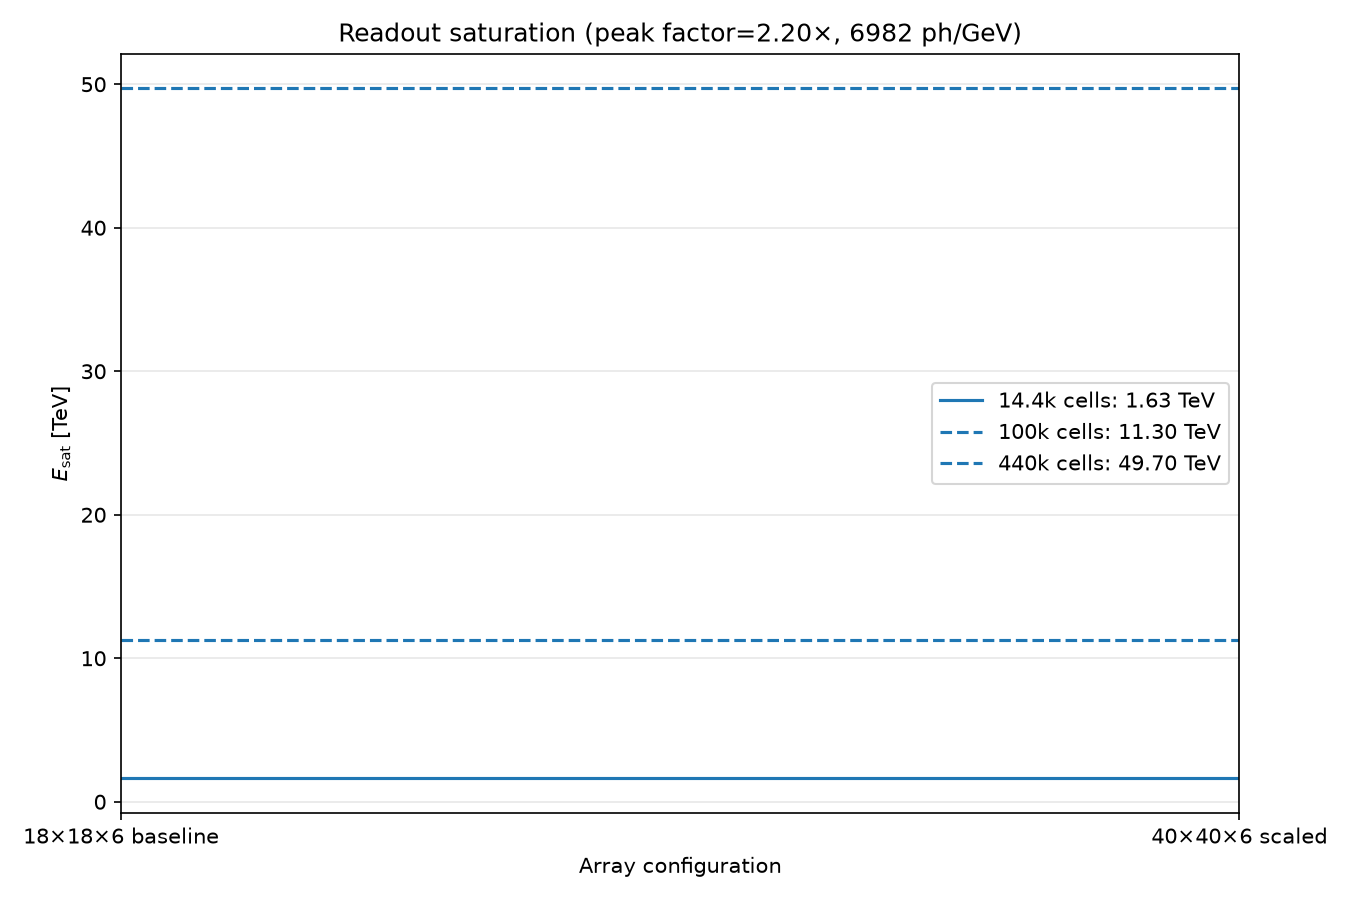
\includegraphics[width=0.85\linewidth]{saturation_energy.png}
\caption{SiPM saturation energy for the baseline 18$\times$18$\times$6 array using regenerated calibration ($6982$~photons~GeV$^{-1}$ filter ON), peak factor $\sim$2.2$\times$, PDE~$=0.25$, and $\eta=0.2$, for three microcell densities.}
\label{fig:saturation_vs_array}
\end{figure}

\subsection{Background Rejection}

Charged cosmic rays outnumber astrophysical gamma rays by several orders of magnitude and thus represent the dominant source of background for space-based gamma-ray observatories. To suppress these events, the telescope employs an anti-coincidence detector (ACD) system modeled after the successful design of the Fermi-LAT instrument.

The ACD is composed of segmented plastic scintillator panels coupled to SiPM readouts, covering all six faces of the LXe detector. When a charged particle traverses the instrument, it produces scintillation light in the ACD, generating a veto signal in coincidence with the main detector response. Events with simultaneous ACD activity are rejected in real time, ensuring that only neutral gamma-ray interactions are retained for further reconstruction. The segmentation mitigates self-veto effects caused by secondary shower particles, which become increasingly relevant at multi-TeV energies.

This design provides high charged-particle rejection efficiency without sacrificing the instrument’s nearly omnidirectional acceptance, and thus represents a critical component of the overall detection principle. Monte Carlo proton background events (FTFP\_BERT hadronic physics) produce broader, more isotropic six-face patterns than gamma rays; face-anisotropy separates the populations with median ratio $\sim 2.6\times$ (proton/gamma, Figure~\ref{fig:background_rejection}).

\begin{figure}[htbp]
\centering
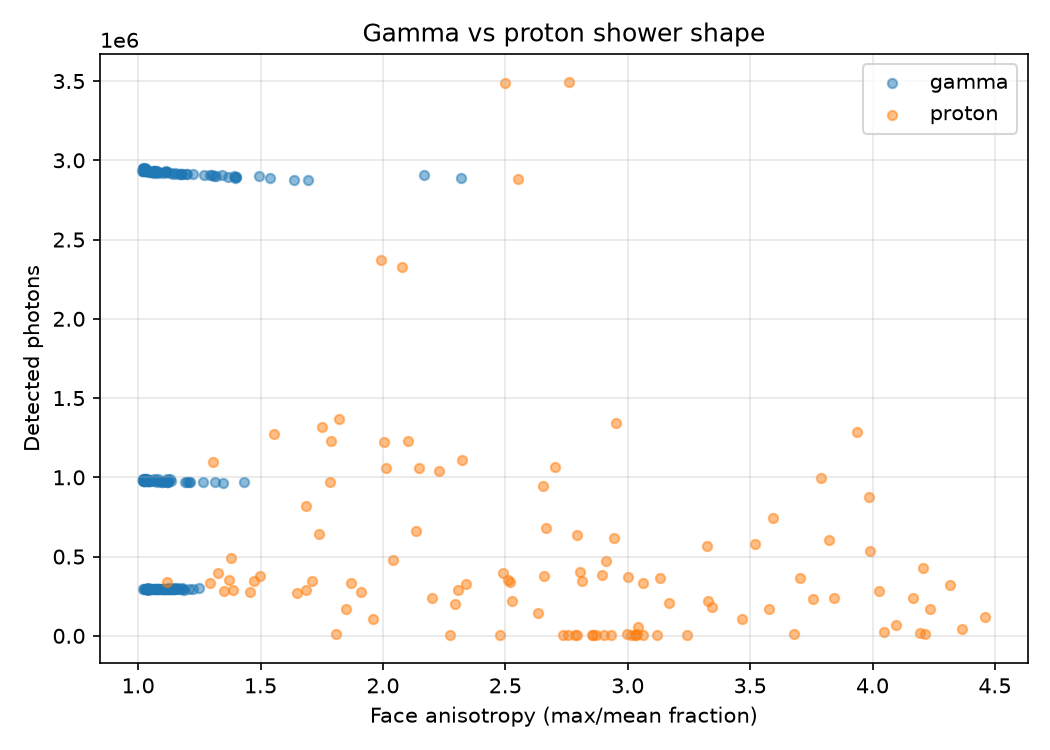
\includegraphics[width=0.75\linewidth]{background_rejection.png}
\caption{Simulated gamma-ray vs.\ proton separation in face-anisotropy vs.\ detected-photon space.}
\label{fig:background_rejection}
\end{figure}

\subsection{Effective Area}

The geometric effective area $A_\mathrm{eff}$ for normally incident $\gamma$ rays is estimated from a plane-source Monte Carlo (1.6$\times$1.6~m$^2$ throw area, 200~GeV, 1000 primaries). Interacting events are identified by LXe energy deposition above threshold; $A_\mathrm{eff} = (N_\mathrm{int}/N_\mathrm{throw})\,A_\mathrm{throw} \approx 0.9$~m$^2$ (Figure~\ref{fig:effective_area}).

\begin{figure}[htbp]
\centering
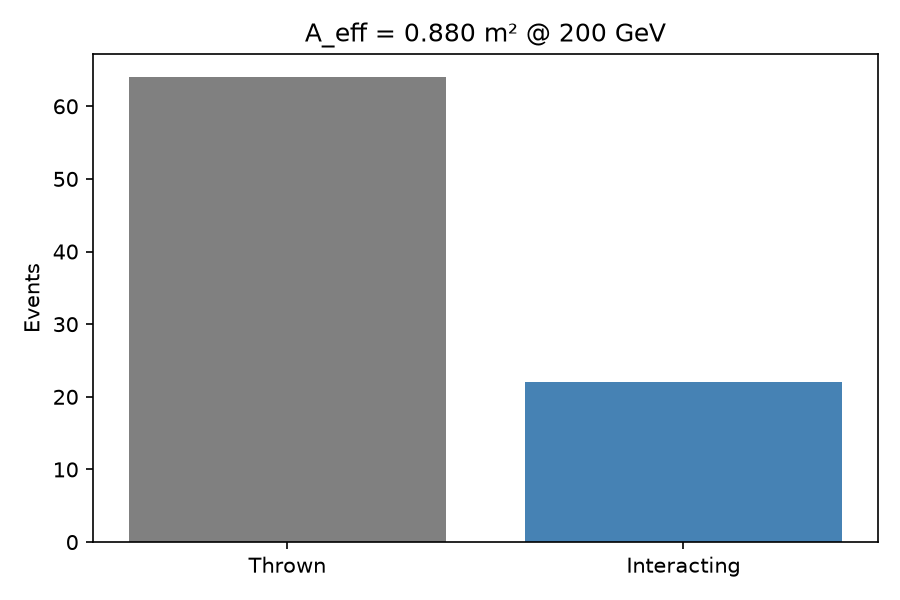
\includegraphics[width=0.65\linewidth]{effective_area.png}
\caption{Effective area estimate from plane-source Geant4 simulation.}
\label{fig:effective_area}
\end{figure}

\section{Discussion}

\subsection{Comparison with \textit{Fermi}-LAT and CTA}

Table~\ref{tab:instrument_compare} summarizes how the simulated LXe Cherenkov concept compares with operating facilities. The cubic geometry provides nearly $4\pi$ acceptance within the LXe volume, while space-borne \textit{Fermi}-LAT maintains a wide survey FoV ($\sim 2.4$~sr) but pair-track angular resolution degrades below $\sim 0.1^\circ$ at 10~GeV and its calorimeter depth limits containment above a few hundred GeV \cite{Atwood2009,Ackermann2012}. Ground-based CTA achieves superior angular resolution ($\sim 0.05^\circ$) and TeV sensitivity but with narrow FoV and $< 15\%$ duty cycle \cite{CTAO_performance_2025}. The simulation demonstrates that photon-counting energy resolution at 215~GeV approaches the Poisson limit ($\lesssim 1\%$), competitive with \textit{Fermi}-LAT above 1~GeV and advantageous relative to IACT energy resolution, while readout saturation presently caps reliable event energy near 1.6~TeV for baseline SiPMs.

\begin{table}[htbp]
\centering
\caption{Instrument comparison (representative published values vs.\ this simulation).}
\label{tab:instrument_compare}
\begin{tabular}{lccc}
\toprule
Metric & \textit{Fermi}-LAT & CTA & LXe concept (sim.) \\
\midrule
Energy range & 20~MeV--300~GeV & 20~GeV--300~TeV & 50~GeV--1.6~TeV$^{\rm a}$ \\
$\sigma_E/E$ @ 215~GeV & $\sim 9\%$ @ 1~GeV & moderate & $\sim 0.50\%$ \\
Angular resolution & $\sim 0.6^\circ$ @ 1~GeV & $\sim 0.05^\circ$ & $\sigma_{68}\approx 0.13^\circ$ vertical (Route~A) \\
FoV / acceptance & 2.4~sr survey & $\sim 10$~deg & $\lesssim 1~{\rm m}^3$ cube \\
Duty cycle & $>90\%$ & $\lesssim 15\%$ & space (TBD) \\
\bottomrule
\end{tabular}
\vspace{0.2cm}
\footnotesize{$^{\rm a}$Saturation-limited with 14{,}400-cell SiPMs; geometric containment extends higher.}
\end{table}

\subsection{Systematic Uncertainties}

Regenerated results supersede earlier draft numbers (9215 vs.\ 9245.6~photons~GeV$^{-1}$, 0.79 vs.\ 0.90~TeV saturation) that arose from broken multithreaded output in the legacy Geant4 build; old and new values are tabulated in \texttt{docs/data\_provenance.md}. Remaining systematics include: (i)~\textit{LXe optical model}---Sellmeier $n(\lambda)$, absorption, and Rayleigh data propagate directly into Cherenkov yield and transport; (ii)~\textit{shower fluctuations}---finite MC statistics and cascade variance dominate energy resolution at fixed $E$; (iii)~\textit{SiPM granularity}---1~cm$^2$ pixels and 25\% PDE approximate commercial VUV SiPMs but omit pixel crosstalk and afterpulsing; (iv)~\textit{filter model}---TMM transmission is idealized (no surface roughness or angular dependence); (v)~\textit{geometry leakage}---1~m$^3$ LXe may not fully contain the highest-energy showers. Future work will quantify each term with dedicated macro campaigns and covariance propagation into reconstructed observables.

\section{Engineering Feasibility}\label{sec:feasibility} 

Despite the validation of the LXe Cherenkov detector's excellent performance through Geant4 simulations, its realization in a space environment involves multiple significant technical challenges and engineering trade-offs.

\subsection{Telescope Material}
The selection of materials for a space-based Liquid Xenon Cherenkov telescope is a critical engineering challenge, demanding a careful balance among cryogenic stability, structural integrity, and the minimization of high-energy gamma-ray interaction. The telescope requires a robust cryogenic design to maintain the LXe medium at a stable 165K and ensure exceptional temperature uniformity, which is vital for the precise measurement of the medium's refractive index and accurate direction reconstruction.

The outer framework must provide mechanical support to withstand launch loads and protect the cryogenic vessel. Titanium alloys, specifically Ti-6Al-4V, are the standard choice for the external frame due to their superior strength-to-weight ratio, high specific strength, and proven compatibility with extreme cryogenic environments.

The inner vessel is the core structural component, and its material choice directly impacts both the $\gamma$-ray detection performance and the thermal stability of the LXe medium. The fundamental conflict in material selection lies between maximizing thermal conductivity to ensure temperature uniformity and selecting a low atomic number ($\text{Z}$) to minimize $\gamma$-ray pre-interaction. Any structural material surrounding the LXe medium acts as a potential source of background, where incident $\gamma$-rays can be weakened or misdirected primarily through the Photoelectric Effect, Compton Scattering, and Pair Production. Since the cross-sections for these processes scale strongly with the material's Z, density, and thickness, the guiding principle for superior physics performance is to use low-$\text{Z}$ and thin-walled materials to maximize $\gamma$-ray penetration and preserve incident information.Several candidates populate this trade-space. Oxygen-Free High-Conductivity Copper (OFHC Cu, Z=29) offers exceptionally high thermal conductivity (approximately $400\text{ W/m}\cdot\text{K}$ at 165 K) and chemical inertness. This high conductivity is crucial for maintaining the stringent thermal uniformity required for stable refractive index and precise direction reconstruction. However, copper’s high $\text{Z}$ value significantly increases the probability of pre-interaction, introducing undesirable background. In contrast, High-Purity Aluminum ($\text{Al}, \text{Z}=13$) presents a clear mass advantage and a significantly lower interaction rate than copper, making it favorable for $\gamma$-ray transparency. Extending the low-$\text{Z}$ principle, Beryllium ($\text{Be}, \text{Z}=4$) offers the lowest radiation interaction rate of any common engineering material, while Glass Fiber Reinforced Plastic ($\text{GFRP}$), a low-$\text{Z}$ composite, maintains low interaction while potentially offering mechanical strength. The major drawback of these low-$\text{Z}$ materials (Aluminum, Beryllium, and $\text{GFRP}$) is their comparatively lower thermal conductivity relative to copper, which complicates the engineering task of achieving the necessary thermal uniformity for high-resolution detection. Beryllium also presents challenges related to cost and toxicity, and $\text{GFRP}$’s low thermal conductivity and outgassing must be carefully assessed. Therefore, the final material selection represents a critical trade-off between superior thermal stability (for measurement precision) afforded by high-conductivity materials and minimal $\gamma$-ray pre-interaction (for high efficiency and background suppression) provided by low-$\text{Z}$ materials. Future work to solve this challenge must concentrate on exploring innovative composite structures and thickness optimization to provide an effective solution that meets all demanding requirements simultaneously.

\subsection{Temperature Control}
The second paramount challenge lies in the design of a robust, long-duration Space Cryocooler System necessary to maintain the large LXe volume at a precise and stable $165\text{ K}$ throughout the multi-year mission. The total thermal load is fundamentally determined by the sum of conductive heat leak, defined by Fourier's law ($Q_{\text{cond}} = kA\frac{\Delta T}{L}$), and radiative heat leak, quantified by the Stefan-Boltzmann law ($Q_{\text{rad}}=\sigma\epsilon A(T_{\text{hot}}^4-T_{\text{cold}}^4)$). This necessitates a trade-off among various cooling mechanisms. While passive radiative cooling offers zero power consumption and is leveraged by the stable L2 environment, and stored cryogen systems simplify operation, the required mission duration and stability necessitate an active system. After evaluating mechanical options (Stirling, Pulse-Tube, and Joule-Thomson), the Pulse-Tube Cryocooler (PTC) is the recommended solution. This technology, exemplified by its use on the James Webb Space Telescope (JWST) \cite{Gardner2023JWST}, is favored for its long operational lifespan, high reliability, and, crucially, its minimal vibration output compared to Stirling coolers. To manage the thermal load during the ascent phase, the LXe will be pre-cooled to approximately $150\text{ K}$ using high-efficiency Multi-Layer Insulation ($\text{MLI}$) and the system's thermal inertia. Once in orbit, the primary engineering constraints shift to active cooling reliability and power consumption, as the PTC must operate continuously within the spacecraft's strict power budget. Moreover, the entire cooling system must be meticulously thermally and mechanically decoupled from the sensitive LXe enclosure. This is vital to prevent residual thermal cycling and mechanical noise from propagating into the active volume, which would compromise the Cherenkov light collection and the precision of the density-driven reconstruction.

\subsection{Auxiliary Module}

The Auxiliary Module is designed as a physically separate subsystem from the primary LXe enclosure in order to minimize parasitic heat transfer, which could otherwise complicate the thermal management of the main detector volume. By spatially isolating the auxiliary components, the module ensures that heat generated by computing, communication, or power management systems does not perturb the highly sensitive temperature-controlled LXe environment. 

The module houses several critical systems, including the onboard computer for data processing and control, the communication system for telemetry and command uplink/downlink, and the power management subsystem responsible for distributing energy to both the auxiliary and primary modules. To enhance the operational reliability in a space environment, the Auxiliary Module is further equipped with dedicated radiation shielding designed to mitigate the effects of cosmic rays and high-energy particles, thereby protecting delicate electronic components from ionizing radiation damage. 

Overall, this design philosophy balances the need for functional integration with the imperative to maintain thermal and radiation stability in the primary detector, allowing the main LXe system to operate under optimal and predictable conditions while supporting essential spacecraft operations.

\section{Conclusion}

We report a reproducible Geant4~11.3.2 simulation of a 1~m$^3$ liquid-xenon Cherenkov telescope with 1{,}944 interior SiPMs. The regenerated pipeline yields $9781$ detected photons per GeV (filter OFF), $6982$ per GeV (filter ON), $\sigma_E/E \approx 0.50\%$ at 215~GeV, a filter transmission of $\sim 71\%$, and a SiPM peak factor of $\sim$2.2$\times$, implying $E_{\rm sat}\approx 1.63$~TeV for baseline 14{,}400-cell devices. Route~A geometric reconstruction achieves $\sigma_{68}\approx 0.13^\circ$ for vertical incidence. These self-consistent numbers replace earlier draft metrics that could not be reproduced from the archived code.

\begin{acknowledgments}
The authors acknowledge that this work originated from the Johns Hopkins University Summer Program, where the concept of the proposed liquid xenon Cherenkov telescope was first formulated. We are sincerely grateful to Dr. Kelly Lepo (Space Telescope Science Institute) and Mr. Joshua Lake (Pomfret School) for their expert advice and support. We also thank the development teams of MATLAB, Geant4, ParaView, and Cursor for providing essential tools used in this study.
\end{acknowledgments}

\begin{contribution}
J.~Tian conceived the core concept of the proposed gamma-ray telescope and developed all theoretical models and reconstruction algorithms presented in this work. He also wrote the entire \textit{Telescope Design and Performance} section and led the overall scientific analysis. B.~Malool led the research and discussion of the telescope's feasibility and technical challenges, originated the critical design choice to separate the telescope into two distinct modules to minimize thermal transfer and maintain cryogenic stability. She authored the material selection, temperature control system and auxiliary module. Both authors reviewed and approved the final manuscript.
\end{contribution}

\bibliography{citation}{}
\bibliographystyle{aasjournalv7}

\end{document}
